% ---------------------------------------------------------------
% Modelo LaTex para dissertação e tese do programa de Pós Graduação em Ciência da Computação da UFABC
% ---------------------------------------------------------------

\documentclass[
	% -- opções da classe memoir --
	12pt,					% tamanho da fonte
	openright,				% capítulos começam em pág ímpar (insere página vazia caso preciso)
	twoside,					% para impressão em verso e anverso. Oposto a oneside
	a4paper,					% tamanho do papel. 
	% -- opções da classe abntex2 --
	%chapter=TITLE,			% títulos de capítulos convertidos em letras maiúsculas
	%section=TITLE,			% títulos de seções convertidos em letras maiúsculas
	%subsection=TITLE,		% títulos de subseções convertidos em letras maiúsculas
	%subsubsection=TITLE,	% títulos de subsubseções convertidos em letras maiúsculas
	% -- opções do pacote babel --
	english,					% idioma adicional para hifenização
	%french,					% idioma adicional para hifenização
	%spanish,				% idioma adicional para hifenização
	brazil					% o último idioma é o principal do documento
	]{abntex2}

% ---------------------
% Pacotes OBRIGATÓRIOS
% ---------------------
\usepackage{lmodern}				% Usa a fonte Latin Modern			
\usepackage[T1]{fontenc}			% Selecao de codigos de fonte.
\usepackage[utf8]{inputenc}		% Codificacao do documento (conversão automática dos acentos)
\usepackage{lastpage}			% Usado pela Ficha catalográfica
\usepackage{indentfirst}			% Indenta o primeiro parágrafo de cada seção.
\usepackage{color}				% Controle das cores
\usepackage{graphicx,graphicx}	% Inclusão de gráficos
\usepackage{epsfig,subfig}		% Inclusão de figuras
\usepackage{microtype} 			% Melhorias de justificação
% ---------------------
		
% ---------------------
% Pacotes ADICIONAIS
% ---------------------
\usepackage{lipsum}						% Geração de dummy text
\usepackage{amsmath,amssymb,mathrsfs}	% Comandos matemáticos avançados 
\usepackage{setspace}  					% Para permitir espaçamento simples, 1 1/2 e duplo
\usepackage{verbatim}					% Para poder usar o ambiente "comment"
\usepackage{tabularx} 					% Para poder ter tabelas com colunas de largura auto-ajustável
\usepackage{afterpage} 					% Para executar um comando depois do fim da página corrente
\usepackage{url} 						% Para formatar URLs (endereços da Web)
\usepackage{minted}             % Formata códigos

\numberwithin{equation}{subsection}
\let\oldsection\section% Store \section
\renewcommand{\section}{% Update \section
  \renewcommand{\theequation}{\thesection.\arabic{equation}}% Update equation number
  \oldsection}% Regular \section
\let\oldsubsection\subsection% Store \subsection
\renewcommand{\subsection}{% Update \subsection
  \renewcommand{\theequation}{\thesubsection.\arabic{equation}}% Update equation number
  \oldsubsection}% Regular \subsection
% ---------------------
% ---------------------

% ---------------------
% Pacotes de CITAÇÕES
% ---------------------
\usepackage[brazilian,hyperpageref]{backref}	% Paginas com as citações na bibl
\usepackage[alf]{abntex2cite}				% Citações padrão ABNT (alfa)
%\usepackage[num]{abntex2cite}				% Citações padrão ABNT (numericas)
% ---------------------

% Configurações de CITAÇÕES para abntex2
% --- 
% CONFIGURAÇÕES DE PACOTES
% --- 

% ---
% Configurações do pacote backref
% Usado sem a opção hyperpageref de backref
\renewcommand{\backrefpagesname}{Citado na(s) página(s):~}
% Texto padrão antes do número das páginas
\renewcommand{\backref}{}
% Define os textos da citação
\renewcommand*{\backrefalt}[4]{
	\ifcase #1 %
		Nenhuma citação no texto.%
	\or
		Citado na página #2.%
	\else
		Citado #1 vezes nas páginas #2.%
	\fi}%
% ---

% Inclusão de dados para CAPA e FOLHA DE ROSTO (título, autor, orientador, etc.)
% ---
% Informações de dados para CAPA e FOLHA DE ROSTO
% ---
\titulo{Desenvolvimento de Laboratório Virtual: Um Ambiente para o Ensino de Modelagem e Controle de CubeSat}
\autor{Gabriel Alves Silva}
\local{Santo André - SP}
\data{Abril de 2024}
\orientador{Diego Paolo Ferruzzo Correa}
\instituicao{%
  Universidade Federal do ABC -- UFABC
  \par
  Pró-reitoria de Pós-graduação da UFABC 
  \par
  Programa de Pós-Graduação em Engenharia Mecânica}
\tipotrabalho{Dissertação (Mestrado)}
% O preambulo deve conter o tipo do trabalho, o objetivo,
% o nome da instituição e a área de concentração
\preambulo{\textbf{Dissertação de Mestrado} apresentada ao Programa de Pós-Graduação em Engenharia Mecânica (área de concentração: Dinâmica de Sistemas), como parte dos requisitos necessários para a obtenção do Título de Mestre em Engenharia Mecânica.}
% ---

% Inclui Configurações de aparência do PDF Final
%  Configurações de aparência do PDF final
% NÃO ALTERAR!!!

% alterando o aspecto da cor azul
\definecolor{blue}{RGB}{41,5,195}

% informações do PDF
\makeatletter
\hypersetup{
     	%pagebackref=true,
		pdftitle={\@title}, 
		pdfauthor={\@author},
    		pdfsubject={\imprimirpreambulo},
	    pdfcreator={LaTeX with abnTeX2},
		pdfkeywords={abnt}{latex}{abntex}{abntex2}{trabalho acadêmico}, 
		colorlinks=true,       		% false: boxed links; true: colored links
    		linkcolor=blue,          	% color of internal links
    		citecolor=blue,        		% color of links to bibliography
    		filecolor=magenta,      		% color of file links
		urlcolor=blue,
		bookmarksdepth=4
} 
\makeatother
% --- 

% O tamanho da identação do parágrafo é dado por:
\setlength{\parindent}{1.3cm}

% Controle do espaçamento entre um parágrafo e outro:
\setlength{\parskip}{0.2cm}  % tente também \onelineskip

% ---------------------
% Compila o indice
% ---------------------
\makeindex
% ---------------------

% ---------------------
% Configuração Adição de Script
% ---------------------
\usepackage{listings}
\usepackage{color}

\definecolor{dkgreen}{rgb}{0,0.6,0}
\definecolor{gray}{rgb}{0.5,0.5,0.5}
\definecolor{mauve}{rgb}{0.58,0,0.82}

\lstset{frame=tb,
  language=sh,
  aboveskip=3mm,
  belowskip=3mm,
  showstringspaces=false,
  columns=flexible,
  basicstyle={\small\ttfamily},
  numbers=none,
  numberstyle=\tiny\color{gray},
  keywordstyle=\color{blue},
  commentstyle=\color{dkgreen},
  stringstyle=\color{mauve},
  breaklines=true,
  breakatwhitespace=true,
  tabsize=3
}
\lstdefinelanguage{XML}
{
  basicstyle=\ttfamily\footnotesize,
  morestring=[b]",
  moredelim=[s][\bfseries\color{gray}]{<}{\ },
  moredelim=[s][\bfseries\color{gray}]{</}{>},
  moredelim=[l][\bfseries\color{gray}]{/>},
  moredelim=[l][\bfseries\color{gray}]{>},
  morecomment=[s]{<?}{?>},
  morecomment=[s]{<!--}{-->},
  commentstyle=\color{dkgreen},
  stringstyle=\color{blue},
  identifierstyle=\color{red}
}
% ---------------------
\usepackage{pgfgantt}
%%%%%%%%%%%%%%%%%%%%%%%%%%%
%%  INICIO DO DOCUMENTO  %%
%%%%%%%%%%%%%%%%%%%%%%%%%%%
\begin{document}

% Retira espaço extra obsoleto entre as frases.
\frenchspacing

% ----------------------------------------------------------
% ELEMENTOS PRÉ-TEXTUAIS (Capa, Resumo, Abstract, etc.)
% ----------------------------------------------------------
\pretextual

% Capa
% ---
% Impressão da Capa
% ---
  \begin{capa}%
    \begin{figure}[h!]%
        \centering%
        
\includegraphics[scale=1.2]{figs/logo.png}%
      \end{figure}%
    \center
	\ABNTEXchapterfont\large{Universidade Federal do ABC \\  Pró-reitoria de Pós-graduação da UFABC\\ Programa de Pós-Graduação em Engenharia Mecânica}
	%\vspace{1.5cm}

    \vfill
    \ABNTEXchapterfont\bfseries\LARGE\imprimirtitulo
    \vfill

	%\vfill
	\ABNTEXchapterfont\large\imprimirautor
	\vfill
%
	Número de Ordem : XXXX
	
    \large\imprimirlocal, \large\imprimirdata

    \vspace*{1cm}
  \end{capa}
% ---

% Folha de rosto (o * indica que haverá a ficha bibliográfica)
\imprimirfolhaderosto*

% Imprimir Ficha Catalografica
% ---
% Ficha Catalográfica
% ---
% Isto é um exemplo de Ficha Catalográfica, ou ``Dados internacionais de
% catalogação-na-publicação''. Você pode utilizar este modelo como referência. 
% Porém, talvez a biblioteca lhe fornece um PDF
% com a ficha catalográfica definitiva após a defesa do trabalho. Quando estiver
% com o documento, salve-o como PDF no diretório do seu projeto e substitua todo
% o conteúdo de implementação deste arquivo pelo comando abaixo:
%
% \begin{fichacatalografica}
%     \includepdf{fig_ficha_catalografica.pdf}
% \end{fichacatalografica}
\begin{fichacatalografica}
	\vspace*{\fill}					% Posição vertical
	\hrule							% Linha horizontal
	\begin{center}					% Minipage Centralizado
	\begin{minipage}[c]{12.5cm}		% Largura
	
	\imprimirautor
	
	\hspace{0.5cm} \imprimirtitulo  / \imprimirautor. --
	\imprimirlocal, \imprimirdata-
	
	\hspace{0.5cm} \pageref{LastPage} p. : il. (algumas color.) ; 30 cm.\\
	
	\hspace{0.5cm} \imprimirorientadorRotulo~\imprimirorientador\\
	
	\hspace{0.5cm}
	\parbox[t]{\textwidth}{\imprimirtipotrabalho~--~\imprimirinstituicao,
	\imprimirdata.}\\
	
	\hspace{0.5cm}
		1. CubeSat.
		2. Simulação.
        3. Determinação e Controle de Atitude.
        4. Plataforma Virtual.
        5. Código Aberto.
		I. Diego Paolo Ferruzzo Correa.
		II. Universidade Federal do ABC.
		III. Programa de Pós-Graduação em Engenharia Mecânica.
		IV. Desenvolvimento de Laboratório Virtual: Um Ambiente para o Ensino de Modelagem e Controle de CubeSat.\\ 			
	
	\hspace{8.75cm} CDU 02:141:005.7\\
	
	\end{minipage}
	\end{center}
	\hrule
\end{fichacatalografica}
% ---

% Inserir Folha de Aprovação
% ---
% Assinaturas
% ---
% Este é um exemplo de folha de aprovação, elemento obrigatório da NBR
% 14724/2011 (seção 4.2.1.3). Você pode utilizar este modelo até a aprovação
% do trabalho. Após isso, substitua todo o conteúdo deste arquivo por uma
% imagem da página assinada pela banca com o comando abaixo:
%
% \includepdf{folhadeaprovacao_final.pdf}
%
\begin{folhadeaprovacao}

  \begin{center}
    {\ABNTEXchapterfont\large\imprimirautor}

    \vspace*{\fill}\vspace*{\fill}
    \begin{center}
      \ABNTEXchapterfont\bfseries\Large\imprimirtitulo
    \end{center}
    \vspace*{\fill}
    
    \hspace{.45\textwidth}
    \begin{minipage}{.5\textwidth}
        \imprimirpreambulo
    \end{minipage}%
    \vspace*{\fill}
   \end{center}
        
 % Isso na versao final do trabalho!!!       
   Trabalho aprovado. \imprimirlocal, 01 de janeiro de 2024:

   \assinatura{\textbf{Dr. DIEGO PAOLO FERRUZZO CORREA, UFABC \\ Presidente -Interno ao Programa}
   \assinatura{\textbf{Dr. LUIZ DE SIQUEIRA MARTINS FILHO, UFABC} \\ Membro Titular - Examinador Interno ao Programa}
   \assinatura{\textbf{Dr. LEANDRO BARONI, UFABC} \\ Membro Titular - Examinador Externo ao Programa}
   \assinatura{\textbf{Dr. ANTONIO GIL VICENTE DE BRUM, UFABC} \\ Membro Suplente - Examinador Externo ao Programa}
      
   \begin{center}
    \vspace*{0.5cm}
    {\large\imprimirlocal}
    \par
    {\large\imprimirdata}
    \vspace*{1cm}
  \end{center}
  
\end{folhadeaprovacao}
% ---

% Dedicatória
% ---
% Dedicatória
% ---
\begin{dedicatoria}
   \vspace*{\fill}
   \centering
   \noindent
   \textit{ Aos verme que roeu as frias carnes de meu cadáver.} \vspace*{\fill}
\end{dedicatoria}
% ---

% Agradecimentos
% ---
% Agradecimentos
% ---
\begin{agradecimentos}


Agradeço ao meu orientador, XXXXXXXXX, por todos os conselhos, pela paciência e ajuda nesse período.

Aos meus amigos ...

Aos professores ...

À XXXXXX pelo apoio financeiro para realização deste trabalho de pesquisa.

\end{agradecimentos}
%% ---

% Epígrafe
% ---
% Epígrafe
% ---
\begin{epigrafe}
    \vspace*{\fill}
	\begin{flushright}
		\textit{``Não sei o que, \\
		          não sei o que,\\
                  não sei o que lá.''\\
		          (Autor Desconhecido)}
	\end{flushright}
\end{epigrafe}
% ---

% Resumo e Abstract
% ---
% RESUMOS
% ---

% RESUMO em português
\setlength{\absparsep}{18pt} % ajusta o espaçamento dos parágrafos do resumo
\begin{resumo}

O presente projeto tem como objetivo principal o desenvolvimento de uma plataforma virtual \textit{open-source} voltada para a simulação da dinâmica de um \textit{CubeSat,} com especial ênfase nos elementos críticos do subsistema de determinação e controle de atitude, proporcionando uma interface gráfica intuitiva. Para alcançar essa meta, pretende-se elaborar roteiros detalhados partindo da instalação e configuração das aplicações computacionais, seguindo para a modelagem físico-matemática do \textit{CubeSat}, sensores e atuadores em \textit{Extensible Markup Language (XML)}, a aplicação de técnicas de determinação e controle de atitude com auxilio de \textit{Python, C++ }, assim como a representação de um ambiente espacial virtual interligados pelo \textit{JSBSim}, e \textit{FlightGear}.

Considerando a importância do estudo experimental na engenharia, a plataforma \textit{CubeSat} foi concebida com a meta inicial de facilitar a interação dos estudantes universitários com o espaço e a tecnologia. No entanto, o desenvolvimento e lançamento de um \textit{CubeSat} são tarefas desafiadoras, envolvendo recursos consideráveis. O custo associado, notadamente na casa dos milhões de reais para uma única missão, pode representar uma parcela significativa do orçamento institucional, exemplificado pelos 1\% do orçamento total da Universidade Federal do ABC (UFABC) em 2020. Nesse contexto, o projeto propõe uma solução intermediária.

Guiado pela missão de despertar a vocação científica, inserir estudantes em atividades de pesquisa e aprimorar o desempenho dos alunos na engenharia, o projeto alinha-se às transformações educacionais aceleradas pela pandemia de COVID-19. Utilizando aplicações \textit{open-source} para modelagem, programação e simulação, a proposta não apenas visa desenvolver uma ferramenta técnica avançada, mas principalmente cultiva uma abordagem educacional que promove a participação ativa dos estudantes na exploração do espaço e na engenharia aeroespacial.

Espera-se que o projeto, ao atingir os objetivos propostos, resulte em uma plataforma funcional para desenvolvimento colaborativo, contribuindo significativamente para a formação prática dos estudantes de engenharia aeroespacial, ao facilitar a exploração do espaço de maneira acessível e inovadora.


 \textbf{Palavras-chaves}: CubeSat. Simulação. Determinação e Controle de Atitude. Plataforma virtual. Código Aberto.
\end{resumo}

% ABSTRACT in english
\begin{resumo}[Abstract]
 \begin{otherlanguage*}{english}
 	
 The main objective of this project is the development of an open-source virtual platform aimed at simulating the dynamics of a CubeSat, with a special emphasis on the critical elements of the attitude determination and control subsystem, providing an intuitive graphical interface. To achieve this goal, we intend to elaborate detailed guides starting from the installation and configuration of computational applications, followed by the physical-mathematical modeling of the CubeSat, sensors, and actuators in Extensible Markup Language (XML), the application of attitude determination and control techniques with the help of Python and C++, as well as the representation of a virtual space environment interconnected by JSBSim and FlightGear.
 
 Considering the importance of experimental study in engineering, the CubeSat platform was conceived with the initial goal of facilitating the interaction of university students with space and technology. However, developing and launching a CubeSat is a challenging task involving considerable resources. The associated costs, notably in the millions of reais for a single mission, can represent a significant portion of the institutional budget, exemplified by the 1% of the total budget of the Federal University of ABC (UFABC) in 2020. In this context, the project proposes an intermediate solution.
 
 Guided by the mission to awaken scientific vocation, involve students in research activities, and improve student performance in engineering, the project aligns with the educational transformations accelerated by the COVID-19 pandemic. Using open-source applications for modeling, programming, and simulation, the proposal not only aims to develop an advanced technical tool but also cultivates an educational approach that promotes active student participation in space exploration and aerospace engineering.
 
 It is expected that the project, upon achieving its proposed objectives, will result in a functional platform for collaborative development, significantly contributing to the practical training of aerospace engineering students by facilitating space exploration in an accessible and innovative manner.

   \vspace{\onelineskip}
 
   \noindent 
   \textbf{Keywords}:     cubeSat. simulation. attitude determination and control. virtual platform. opensource.
 \end{otherlanguage*}
\end{resumo}

% Lista de ilustrações
\pdfbookmark[0]{\listfigurename}{lof}
\listoffigures*
\cleardoublepage

% Lista de tabelas
\pdfbookmark[0]{\listtablename}{lot}
\listoftables*
\cleardoublepage


% Lista de abreviaturas e siglas
% Ordem Alfabética
\begin{siglas}
\item[ADCS] Sistema de Determinação e Controle de Atitude (\textit{Attitude Determination and Control System})
 \item[CGEE] Centro de Gestão e Estudos Estratégicos
 \item[CSLI] Iniciativa de lançamento do CubeSat  (\textit{CubeSat Launch Initiative})
 \item [EDO] Equação Diferencial Ordinária
 \item[IGRF] Campo de Referência Geomagnético Internacional (\textit{International Geomagnetic Reference Field})
  \item[INPE] Instituto Nacional de Pesquisas Espaciais
  \item[J2000] Data Juliana em 1 de Janeiro de 2000
  \item[JPL] Laboratório de Propulsão a Jato (\textit{Jet Propulsion Laboratory})
  \item[LEO] Órbita Terrestre Baixa (\textit{Low Earth Orbit})
 \item[MarsCo] (\textit{Mars Cube One})
  \item[NASA] Administração Nacional da Aeronáutica e Espaço (\textit{National Aeronautics and Space Administration})
  \item[NEO] Objeto Próximo da Terra (\textit{Near-Earth Object})  
  \item[PID] Proporcional Integral Derivativo
  \item[REQ] Requisito
  \item[ROS] sistema operacional de robôs (\textit{Robot Operating System})
  \item[RPM] Rotações Por Minuto
  \item[SCFC] Sistema de Coordenadas Fixo no Corpo
  \item[SCGI] Sistema de Coordenadas Geocêntrico-Equatorial Inercial
  \item[SCO] Sistema de Coordenadas Orbital]
  \item[SDF] Formato de Descrição de Simulação (\textit{Simulation Description Format})
  \item[TRIAD] Determinação de Atitude Triaxial (\textit{TRIaxial Attitude Determination})  
  \item[VE] Veículo Espacial  
  \item[URDF] Formato de Descrição de Robôs  Unificado (\textit{Unified Robotics Description Format}) 
  \item[UT] Horário Universal  
\end{siglas}

% Lista de símbolos
\begin{simbolos}
	\item[$\vec{a}$] Aceleração Linear
    \item[B] Base Ortonormal do SCFC
    \item[$\vec{b}$] Versor da Base B
    \item[$C_j$] Matriz de Cossenos Diretores para uma Rotação Elementar sobre o eixo j 
    \item[$C^{B/A}$] Matriz de Transformação de Coordenadas de A para B 
    \item[E] Matriz Antissimétrica do Eixo de Euler
    \item[$\vec{e}$] Eixo de Euler
    \item[$\vec{e}_r$] Eixo Radial
    \item[$\vec{e}_s$] Eixo Transversal
    \item[$e_j$] componente no eixo j do eixo de Euler
    \item[$\vec{F}$] Força
    \item[f] Coeficiente de Viscosidade
    \item[G] Constante Gravitacional Universal
    \item[$\vec{H}$] Momento Angular da Órbita
    \item[$H_j$] Componente j do Momento Angular
    \item[I] Base Ortonormal do SCGI; Matriz Identidade
    \item[$\vec{i}$] Versor da Base I
    \item[J] Matriz de Inercia, Momento de Inercia
    \item[$K_{cr}$] Ganho Crítico
    \item[$K_P$] Ganho Proporcional
    \item[m] Massa
    \item[$N$] Torque
    \item[$N_{em}$] Torque Eletromagnético
    \item[$N_0$] Torque Eletromagnético máximo
    \item[$N_c$] Torque de Coulomb
    \item[O] Base Ortonormal do SCO
    \item[$\vec{o}$] Versor da Base O
    \item[P] Período
    \item[$P_{cr}$] Período Crítico
    \item[Q] Matriz Antissimétrica do Quatérnio
    \item[q] Quatérnio
    \item[R] Matriz de Rotação, Raio
    \item[$\vec{r}$] vetor distância
    \item[r] Razão entre $s$ e $s_{max}$ 
    \item[s] Velocidade de Rotação
    \item[$s_{max}$] Velocidade de Rotação Máxima
    \item[$\vec{v}$] Velocidade Linear
    \item[T] Torque
    \item[$T_i$] Período Integrativo
    \item[$T_d$] Período Derivativo
    \item[t] tempo
    \item[$X_{ct}$] Ciclo de Trabalho   
    \item[$\alpha$] Aceleração Angular
    \item[$\theta$] Ângulo, Arfagem
    \item[$\mu$] Parâmetro Gravitacional
    \item[$\rho$] Dimensão em um Eixo
    \item[$\Upsilon$] Equinócio Vernal
    \item[$\phi$] Rolamento
    \item[$\psi$] Guinada
    \item[$\vec{\omega}$] Velocidade angular
    \item[$\omega_0$] Movimento Médio da órbita
    \item[$\vec{\omega}^b_{ib}$] Velocidade Angular de SCFC em relação ao SCGI visto no SCFC
    \item[$\vec{\omega}^o_{io}$] Velocidade Angular de SCO em relação ao SCGI visto no SCO
    \item[$\vec{\omega}^b_{ob}$] Velocidade Angular de SCFC em relação ao SCO visto no SCFC
\end{simbolos}


% Inserir o SUMÁRIO
\pdfbookmark[0]{\contentsname}{toc}
\tableofcontents*
\cleardoublepage

% ----------------------------------------------------------
% ELEMENTOS TEXTUAIS (Capítulos)
% ----------------------------------------------------------
\textual
% Elementos textuais com numeração arábica
\pagenumbering{arabic}
% Reinicia a contagem do número de páginas
\setcounter{page}{1}

% Inclui cada capitulo da Dissertação
% ----------------------------------------------------------
% Introdução 
% Capítulo sem numeração, mas presente no Sumário
% ----------------------------------------------------------

\chapter*[Introdução]{Introdução}
\addcontentsline{toc}{chapter}{Introdução}

A plataforma CubeSat emergiu como uma alternativa valiosa para países em desenvolvimento ampliarem seu acesso ao espaço. No caso do Brasil, desde 2014, a Agência Espacial Brasileira (AEB) tem colaborado com institutos de pesquisa e universidades na utilização de CubeSats, \cite{Santos2018}. Diferentemente do contexto dos Estados Unidos, onde os CubeSats são frequentemente empregados como projetos estudantis, no Brasil, o desenvolvimento desses satélites muitas vezes se torna uma parte significativa do programa espacial do país.

No entanto, o desenvolvimento e lançamento de um CubeSat não são tarefas trivialmente acessíveis, demandando recursos consideráveis. O custo associado, aproximadamente R\$ 2.921.129,50 para uma única missão \cite{CGEE2018}, pode representar uma parcela significativa do orçamento de uma instituição de ensino, como exemplificado pelos 1\% do orçamento total da Universidade Federal do ABC (UFABC) em 2020 \cite{wikipedia2023}.

Essa realidade destaca a dificuldade em atingir os objetivos iniciais dos CubeSats, que incluíam proporcionar aos estudantes universitários a oportunidade de interagir com o espaço e a tecnologia relacionada. Diante desse cenário, surge a necessidade premente de encontrar uma solução intermediária que permita o treinamento, ensino e experimentação de forma eficaz para estudantes de engenharia aeroespacial e áreas afins.

Uma alternativa promissora para preencher essa lacuna prática é a utilização de aplicações de modelagem, programação e simulação. Contudo, a escolha entre softwares proprietários e open-source torna-se crucial, considerando os custos e a praticidade. Para contornar essas questões, exemplos de sucesso, como a Robotic Academy no ensino de robótica, demonstram a viabilidade de plataformas web de educação gratuita e aberta que facilitam o aprendizado prático \cite{canas2020ros}.

Nesse contexto, o presente projeto de pesquisa propõe a criação de um laboratório virtual utilizando ferramentas open-source. Este laboratório abrangerá modelagem, programação, controle e simulação de sensores, ambiente espacial e atuadores, focando especificamente na plataforma CubeSat.

Além disso, o cenário global atual, marcado pela pandemia de COVID-19, acelerou a adoção de métodos de ensino remoto. Estratégias como o home office e o ensino a distância redefiniram as fronteiras entre o mundo digital e o real, proporcionando uma nova perspectiva para a educação. Este projeto se alinha a essas transformações, oferecendo uma solução educacional híbrida e acessível, que integra a visualização do comportamento mecânico de modelos de CubeSats, experimentação em ambientes virtuais e reais, direcionada a estudantes de engenharia aeroespacial, controle, mecânica, professores e entusiastas \cite{bolu2020engineering}.


\section*{Motivação}\label{sec:Motivação}
\addcontentsline{toc}{section}{Motivação}

Em diversas áreas da engenharia, o estudo experimental é fundamental para o desenvolvimento de habilidades práticas essenciais para a resolução eficiente de problemas futuros. Os laboratórios híbridos surgem como uma abordagem acessível, possibilitando uma interação iterativa entre o mundo real e virtual, local e a distância. 

Guiado pela missão de despertar a vocação científica e incentivar novos talentos entre estudantes de graduação, bem como contribuir significativamente para a formação e inserção desses estudantes em atividades de pesquisa, desenvolvimento tecnológico e inovação.

Esta proposta visa incorporar práticas e tecnologias de ensino híbrido para aprimorar o desempenho dos alunos na engenharia, proporcionando um contato prático abrangente que os laboratórios tradicionais muitas vezes não conseguem oferecer.

Não somente ao se desenvolver uma ferramenta técnica avançada, mas principalmente ao se cultivar uma abordagem educacional que promova a participação ativa dos estudantes na exploração do espaço e na engenharia aeroespacial, alinhando-se assim aos princípios fundamentais da formação acadêmica e científica.


\section*{Objetivos}\label{sec:objetivos}
\addcontentsline{toc}{section}{Objetivos}


\subsection*{Objetivo Geral}\label{sec:Objetivo Geral}
\addcontentsline{toc}{section}{Objetivo Geral}

\begin{itemize}
    \item Criar uma plataforma virtual open-source com capacidade de simulação da dinâmica de um CubeSat, enfocando os elementos cruciais do subsistema de determinação e controle de atitude, e proporcionando uma interface gráfica intuitiva.
\end{itemize}

\subsection*{Objetivos Específicos}\label{sec:Objetivos Específicos}
\addcontentsline{toc}{section}{Objetivos Específicos}
\begin{itemize}
    \item Redigir um Script de Instalação e Configuração das Aplicações Computacionais.
    \item Criar modelo físico-matemático e 3D de um CubeSat.
    \item Criar modelo de Sensores, Atuadores.
    \item Criar algorítimo de determinação e controle de atitude.
    \item Criar ambiente espacial.
    \item  Criar Simulação do CubeSat em ambiente virtual.
    \item Redigir roteiros de modelagem e simulação como experimentos.
\end{itemize}


% PARTE - Define a divisão do documento em partes (Não é obrigatório)
\part{Preparação da pesquisa}

\chapter{Uso de referências bibliográficas}
% ---
O desenvolvimento de um laboratório virtual para o ensino de modelagem e controle de CubeSats é uma tarefa ambiciosa devido à sua extensão, complexidade e natureza multidisciplinar. Requer a integração de tópicos que abrangem desde a mecânica espacial até aplicações de robótica, visualização e simulação, ao mesmo tempo em que mantém um ambiente didático propício ao aprendizado.

O modelo de corpo-rígido em órbita se baseia nas leis de Euler para representação da atitude, sendo eles, matriz de cossenos diretores, ângulos de Euler, ângulo-eixo de Euler e parâmetros de Euler, \textit{i.e.}, quatérnions. Para a visualização da rotação tanto em relação ao corpo quanto em relação a um referencial global são definidos três sistemas de coordenadas seguindo a referência temporal J2000, são eles, o sistema de coordenadas geocêntrico-equatorial inercial, o sistema de coordenadas orbital e o sistema de coordenadas fixo no corpo presentes da literatura \citeonline{zanardi2018}, \citeonline{sellers2000understanding} e \citeonline{wie2008space}. 

Por sua vez o modelo dos Sensores Solar e Magnéticos e Rodas de reação em 3-eixos são adaptados da literatura \citeonline{wertz2012spacecraft} e \cite{baroni2020attitude},  a simplificação desconsiderando ruídos e abstraindo a aquisição dos vetores de posição do sol e o magnético, o atuador utiliza os conceitos de rotação de massa, torque eletromagnético e atrito presente, são arranjadas nos três eixos principais de inércia e se localizam no centro de massa do corpo. O algoritmo de TRIAD utiliza os valores de posição obtidos anteriormente, seguindo a metodologia proposta por \citeonline{hall2003spacecraft} enquanto a técnica de controle PID é implementada conforme descrito por \citeonline{ogata2011engenharia}.

Seguindo a documentação presente em \citeonline{ros2humble}, \citeonline{gazebosim}, \citeonline{sdf} e \citeonline{urdf}. A modelagem do veículo espacial, simplificado como um corpo rígido de configuração 6U, é realizada utilizando URDF (Unified Robotics Description Format) contemplando todos os subsistemas, como sensores solares e magnéticos, rodas de reação e câmera. O ambiente espacial, que inclui o veículo espacial e sua órbita, é obtido por meio de simulação computacional com GNU Octave, e esses valores são utilizados em um SDF (Simulation Description Format) para visualização no Gazebo Simulator. Essa integração dos modelos é facilitada pelo ROS (Robotic Operating System), permitindo a comunicação entre os códigos e os modelos. 




\chapter{Estado da Arte}\label{cap:estArte}

Este capítulo fornece uma revisão dos trabalhos relacionados e resume a contribuição da presente dissertação de mestrado para o estado da arte.

A contribuição primária desta dissertação, como delineada na introdução, é o desenvolvimento de uma plataforma open-source para facilitar a aprendizagem de modelagem, simulação e controle de CubeSats.

Atualmente, os laboratórios virtuais para o ensino de engenharia, como robótica, modelagem, simulação e controle, alcançaram um estágio avançado, principalmente devido à adoção de ferramentas open-source como JSBSim, ROS (Robotic Operating System), Gazebo, FlightGear, Python e Octave.

O JSBSim oferece uma infraestrutura flexível e modular para o desenvolvimento de aeronaves e foguetes, permitindo a integração de diferentes componentes e algoritmos de controle. Por sua vez, o FlightGear é um simulador de voo 3D que proporciona a criação de ambientes virtuais realistas para testes e experimentação. Complementarmente, o Python oferece uma poderosa plataforma de computação numérica para análise e implementação de algoritmos de controle.

Essas ferramentas combinadas possibilitam aos estudantes e pesquisadores explorarem de maneira prática e eficaz os conceitos de modelagem, simulação e controle de CubeSats, contribuindo assim para o avanço da educação e pesquisa na área aeroespacial.

Investigando a literatura é importante ressaltar que as ferramentas do ROS e Gazebo não são tão amplamente utilizadas pela comunidade aeroespacial devido à sua limitação em simular nativamente dimensões espaciais, condições como microgravidade e ambientes sem fricção, elementos essenciais para a análise de CubeSats no espaço.

A seguir, serão discutidos alguns trabalhos relacionados ao uso de ferramentas open-source como JSBSim, Python, ROS, Gazebo, Flightgeat e Octave para o ensino de modelagem ou controle em robótica e CubeSats.

\section*{Trabalhos Relacionados}\label{sec:primTrab}
\addcontentsline{toc}{section}{Trabalhos Relacionados}

\citeonline{lotfi2021use} abordaram um estudo de caso que analisa os potenciais e as limitações das aplicações de código aberto, destacando a modelagem, simulação e análise de um Motor de Corrente Contínua. De acordo com o artigo, cerca de 90\% dos estudantes recorrem ao GNU Octave, Python ficando com 50\%, com essa porcentagem reduzida para 70\% e 35\% respectivamente entre os educadores, reafirmando a preferência da comunidade por essas duas ferramentas abertas. A conclusão dessa primeira parte ressalta que o GNU Octave e o Python oferecem vantagens, como funções e bibliotecas úteis para controle, modelagem e análise numérica.

\citeonline{lotfi2022use}  sintetizaram, em outro estudo de caso, os potenciais e as limitações das aplicações de código aberto na implementação do controle de um manipulador robótico com 2 graus de liberdade. Novamente, o GNU Octave é mencionado por apresentar resultados satisfatórios, mas a falta de um ambiente gráfico para simulações é destacada como uma limitação. Nesse estudo, essa lacuna é superada com o uso do Simulador Gazebo em conjunto com o ROS (Robotic Operating System), embora seja observado que essa ferramenta pode ser menos amigável para iniciantes.

\citeonline{linner2011modeling} descreveram o uso do ROS e Gazebo para a modelagem e simulação de robôs, destacando a utilidade da simulação cinética e dinâmica na avaliação da interação humana com construções robóticas. Embora o artigo se refira principalmente a construções terrestres, o conceito de construção robótica pode ser aplicado também a estruturas como a Estação Espacial Internacional.

Diante do aumento do interesse em manipuladores em órbita, \citeonline{hao2021intelligent} identificaram uma lacuna nas técnicas atuais de modelagem e controle de manipuladores robóticos em ambiente espacial. Sugeriram, portanto, uma arquitetura e plataforma para a realização de estudos nessa área, apresentando uma arquitetura inteligente de GNC (Guiamento, Navegação e Controle) de espaçonave com componentes de IA de ponta para manipulação em órbita. Para treinar a plataforma, tornou-se necessário o acesso a dados confiáveis, os quais foram identificados como indisponíveis ou de custo elevado. Como solução, desenvolveram um simulador visual utilizando a ferramenta Unreal Engine 4, denominado OrVIS (Orbital Visualization). Para testar o sistema, utilizaram o ROS em conjunto com o Gazebo, ressaltando que, como um teste de bancada, não integrava visualização e dinâmica espacial.

\citeonline{kang2019urdf} também reconheceu o aumento na demanda por manipuladores e, consequentemente, por simulações envolvendo esses dispositivos. Considerando que o Gazebo e o ROS são plataformas consolidadas no mercado, ele propôs automatizar a geração de URDFs (Unified Robotic Description Format), o formato utilizado por essas aplicações, a partir dos graus de liberdade dos manipuladores. O URDF é um XML (extensible Markup Language) utilizado para descrever modelos robóticos em ambientes de simulação, especialmente no contexto do ROS. Esse tipo de arquivo contém informações detalhadas sobre a geometria, cinemática, dinâmica e outras propriedades físicas de um robô, incluindo links, juntas, sensores e suas relações espaciais. Esses arquivos desempenham um papel fundamental na modelagem e simulação de robôs em ambientes virtuais, possibilitando que os desenvolvedores visualizem, controlem e testem seus sistemas robóticos antes de implementá-los no mundo real.

\citeonline{udugama2023mini}, é apresentado um projeto de localização e mapeamento simultâneo de um robô móvel utilizando o simulador Gazebo em conjunto com o ROS. É evidente que uma das grandes vantagens desse framework é a diversidade de bibliotecas, plugins e implementações disponíveis para sensores de distância e visualização, odometria, motores e modelagem de robôs.

\citeonline{canas2020ros} é uma plataforma de acesso aberto projetada para a aprendizagem prática de robótica inteligente em cursos de engenharia. Conhecida como Robotics-Academy, ela compreende uma coleção de 18 exercícios apresentando diversos robôs, como carros e drones. A plataforma utiliza o middleware Robotic Operating System (ROS) e o simulador 3D Gazebo, juntamente com a linguagem de programação Python. Dada a natureza multidisciplinar da robótica, a Robotics Academy enfatiza mais os algoritmos do que o middleware.

Como mencionado anteriormente e aprofundado em \citeonline{canas2020open}, destaca-se o curso prático à distância de drones, com ênfase na programação desses Veículos Aéreos Não Tripulados (VANTs). O hardware, que representa o próprio robô, é completamente simulado pelo Gazebo, enquanto os softwares dos drivers para a leitura das informações dos sensores e o controle dos atuadores são fornecidos pelo ROS. Os estudantes desenvolvem algoritmos a partir de templates disponibilizados. Os exercícios abordam uma variedade de tarefas, como navegação por posição, seguir objetos e pouso em um carro em movimento, entre outros.

Um aspecto que merece destaque na Robotics Academy, conforme abordado por \citeonline{roldan2022ros}, é que em uma de suas atualizações mais recentes, foram oferecidas ainda mais opções para distribuição e utilização da plataforma. Inicialmente e até hoje, é possível obter a plataforma baixando seu código-fonte pelo GitHub. No entanto, percebeu-se que a instalação e configuração de pacotes extras eram uma barreira. Para superar esse obstáculo, foram apresentadas duas soluções: a instalação via Docker, que já inclui todas as configurações prévias e pode ser utilizada em sistemas Linux, Windows e MacOS; e também, para eliminar qualquer complicação de configuração por parte do usuário, foi disponibilizada a opção de um webserver pronto para uso, onde a computação ocorre de forma transparente para o usuário. Essas soluções visam maximizar a distribuição entre os interessados.

\citeonline{ramon2023task} propõem várias tarefas de controle espacial para objetos em órbita complexos e com vários graus de liberdade. Apresentam uma framework unificada para simulações de robôs espaciais chamada OnOrbitROS, baseada no ROS. O desenvolvimento e teste de um sistema robótico em seus estágios iniciais são essenciais para reduzir custos, e as simulações estão se tornando cada vez mais comuns para isso. Assim a plataforma OnOrbitROS contribui para a comunidade aeroespacial, que tem sido relutante em adotar o ROS/Gazebo, ao oferecer uma solução que incorpora as qualidades de implementação e teste rápidos que essas ferramentas oferecem.

\citeonline{tavares2019desenvolvimento} desenvolve uma simulação completa de uma missão, do lançamento à inserção de orbita baixa de um Veículo Lançador de Microssatélites utilizando FlightGear, MATLAB e Python, a técnica de controle foi LQR para definir os ganhos do controle PID. 

\citeonline{moness2012automatic} desenvolve um laboratório virtual para o ensino de controle para alunos de graduação de engenharia utilizando a ferramenta FlightGear para o controle de um aeronave Cesna, utiliza-se o lugar das raízes para desenvolver o controle PID e os conceitos são demonstrados em quatro experimentos  permitindo a visualização desses efeitos pelos estudantes.

Esses são apenas alguns exemplos de trabalhos que exploram o uso de ferramentas open-source para o ensino de modelagem e controle de CubeSats. Existem muitos outros estudos e projetos interessantes nessa área, demonstrando o crescente interesse e importância dessas tecnologias na educação e pesquisa espacial.
\chapter{Modelagem Físico Matemática}\label{cap:ferramentas}

\section{Sistemas de Coordenadas e Sistema de Medida de Tempo}\label{sec:3.1.1}

É de fundamental importância para qualquer estudo da mecânica a determinação objetiva dos sistemas de referência, sendo eles o de coordenadas e o de tempo. O parâmetro para essa escolha é a facilitação da formulação, visualização e análise dos fenômenos e resultados.

\subsection{Sistema de Coordenadas Geocêntrico-Equatorial Inercial (SCGI)}\label{sec:3.1.1.1}

Por conta do tempo do fenômeno ser insignificante em relação à variação das direções e origem do sistema de coordenadas, é assumido como hipótese simplificadora que esse sistema é não rotacional e fixo no espaço, \textit{i.e.}, inercial. 

O sistema de coordenadas geocêntrico-equatorial inercial \begin{math}I\end{math} tem como origem o centro de massa da Terra, \textit{i.e.}, geocêntrico, e base composta pelos vetores \begin{math}\{\vec{i}_1,\vec{i}_2,\vec{i}_3\}\end{math}. O eixo $\vec{i}_1$ tem como sentido o equinócio vernal $\Upsilon$, o eixo $\vec{i}_3$ aponta para a normal do plano (fundamental) equatorial terrestre, \textit{i.e.}, o polo Norte celeste e o eixo $\vec{i}_2$ completa a base ortogonal dextrogiro \cite[p.~12-13]{zanardi2018}. Mostrado na Figura~\ref{fig:11}.

\begin{figure}[htpb]
\centering
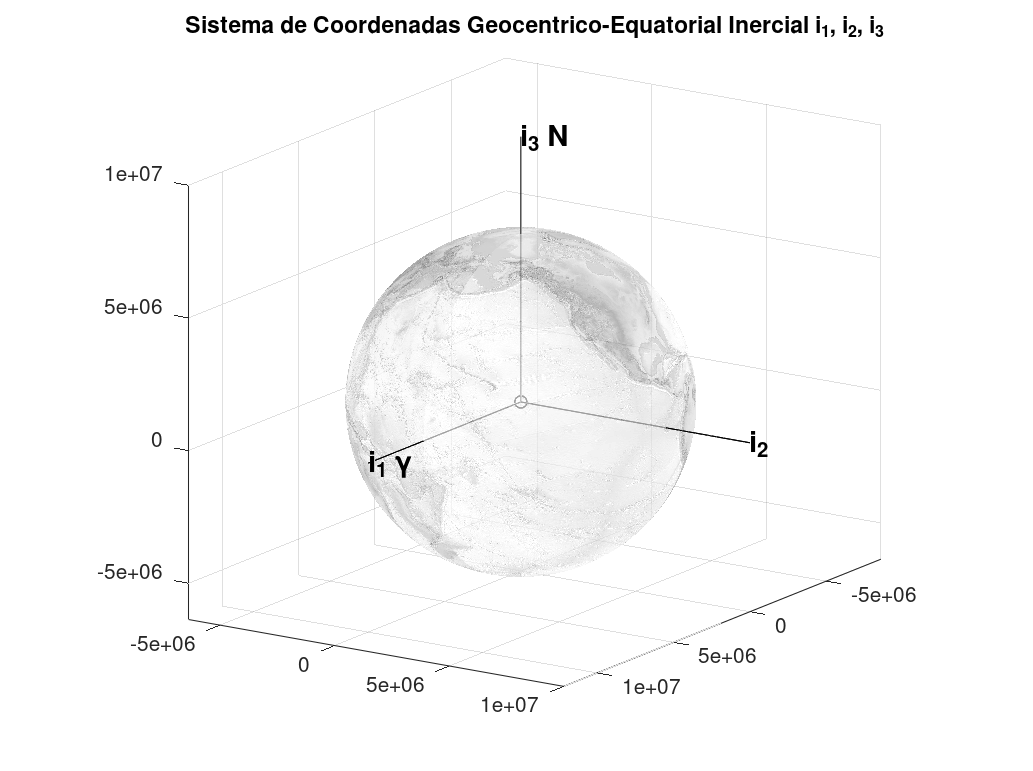
\includegraphics[scale=0.3]{figs/SCGI.png}
\caption{Sistema de Coordenada Geocêntrico-Equatorial Inercial (SCGI)}
\label{fig:11}
\end{figure}

\subsection{Sistema de Coordenadas Orbital (SCO)}\label{sec:3.1.1.2}

O sistema de coordenadas orbital \begin{math}O\end{math} tem como origem o centro de massa do veículo espacial em órbita e base composta pelos vetores \begin{math}\{\vec{o}_1,\vec{o}_2,\vec{o}_3\}\end{math}. O eixo $\vec{o}_3$ aponta em direção ao centro de massa da Terra ou, direção nominal do nadir. O eixo $\vec{o}_2$ tem como direção o oposto do vetor do plano fundamental de órbita do veiculo espacial \cite[p.~26-29]{wertz2012spacecraft}. E o eixo $\vec{o}_1$ aponta para o vetor velocidade nominal ou, a direção nominal da trajetória da órbita. Representado na Figura~\ref{fig:12}.

\begin{figure}[htpb]
\centering
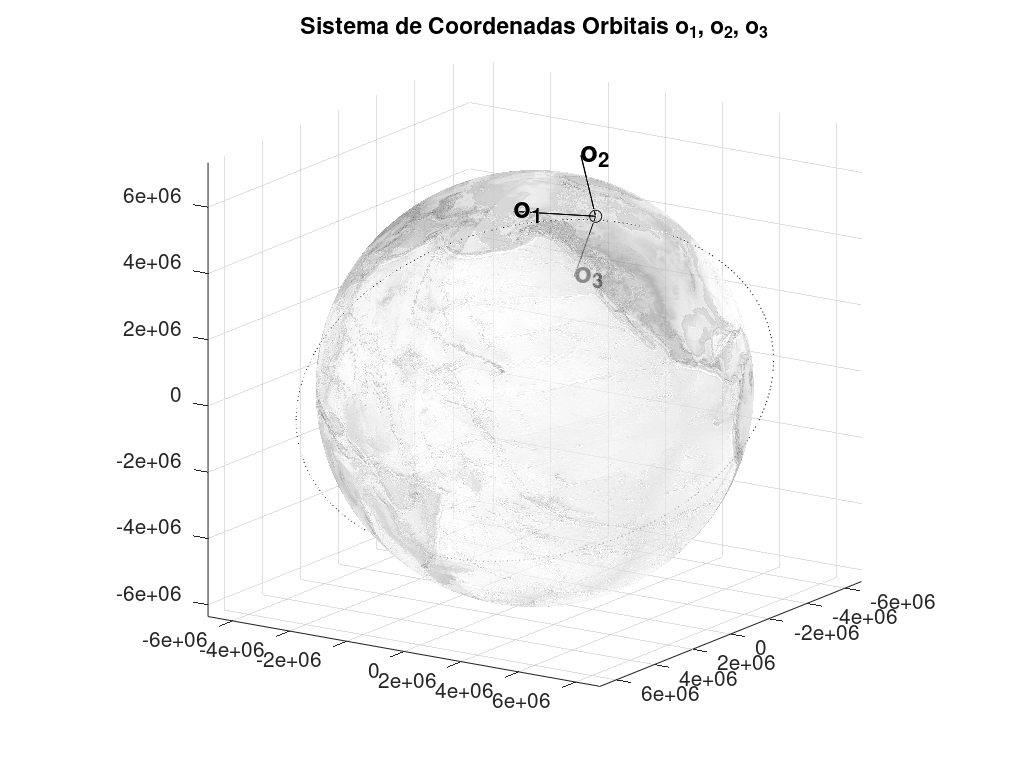
\includegraphics[scale=0.3]{figs/SCO.png}
\caption{Sistema de Coordenada Orbital (SCO)}
\label{fig:12}
\end{figure}

\subsection{Sistema de Coordenadas Fixo no Corpo (SCFC)}\label{sec:3.1.1.3}

O sistema de coordenadas fixo no corpo, \begin{math}B\end{math}, tem como origem o centro de massa do veículo espacial, sua base é composta pelos vetores \begin{math}\{\vec{b}_1,\vec{b}_2,\vec{b}_3\}\end{math}, sendo escolhidos arbitrariamente. É interessante alinhar esses eixos com as direções dos eixos principais de inércia. Escolhendo eixo $\vec{b}_3$ como eixo de Spin, \textit{i.e.}, o eixo de menor momento principal de inércia. Os eixos $\vec{b}_2$, $\vec{b}_1$ o segundo e o terceiro menores momentos principais de inércia \cite[p.~26-29]{wertz2012spacecraft}. Como representado na Figura~\ref{fig:13}.

\begin{figure}[htpb]
\centering
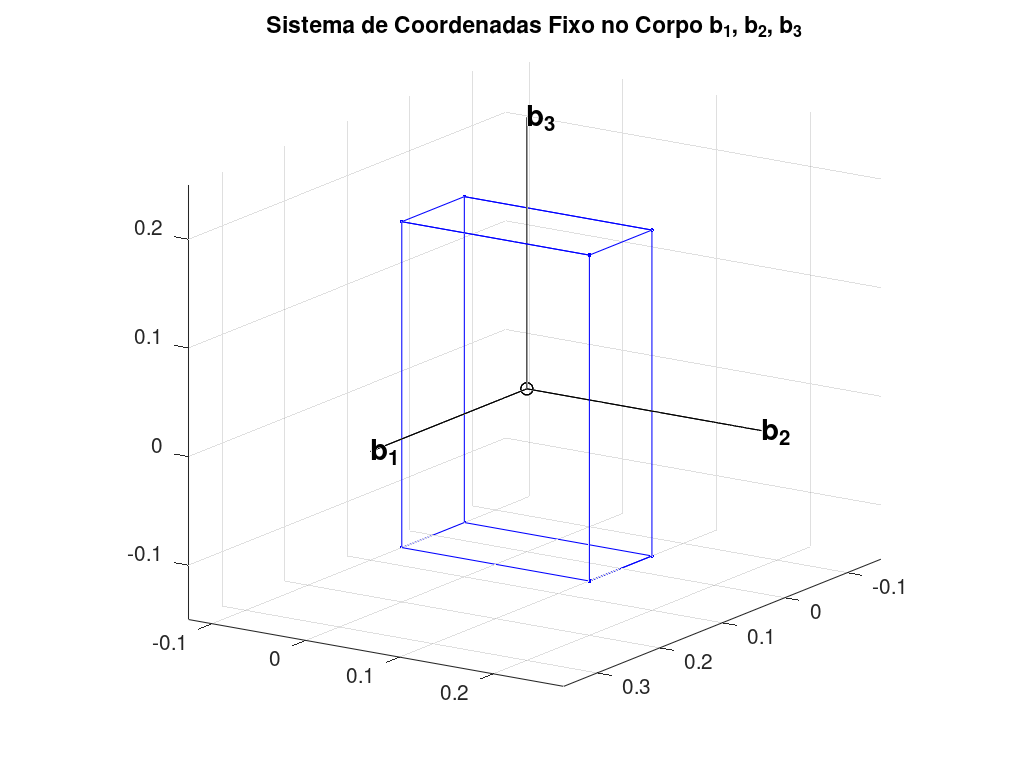
\includegraphics[scale=0.3]{figs/SCBF.png}
\caption{Sistema de Coordenada Fixo no Corpo (SCFC)}
\label{fig:13}
\end{figure}

\subsection{Sistema de Referência de Tempo}\label{sec:3.1.1.4}

A referência para os sistemas de coordenadas descritos acima é o equador médio e o equinócio vernal referente a data Gregoriana de 1º de Janeiro de 2000 às 12 horas U.T. (tempo universal) ou a data Juliana de 2451545. Esse sistema de referência é conhecido como J2000. É a escolha dessa referência que garante que o sistema de coordenadas Geocêntrico-equatorial possa ser considerado não rotacional \cite{schutz2004statistical}.

\section{Mecânica Rotacional}\label{sec:3.1.2}

Nesta seção estuda-se a representação da cinemática rotacional de um corpo rígido. Entende-se que essa formulação é a mesma usada em um modelo de CubeSat. Sendo o principal objetivo descrever a orientação e rotação do corpo.

Existem várias maneiras de representar a atitude de um corpo rígido e a depender do propósito, visualização ou cálculo, umas são mais indicadas que outras. Temos entre elas a matriz de cossenos diretores, os ângulos de Euler, o Eixo-ângulo de Euler e os parâmetros de Euler (Quatérnions).

A formulações a seguir seguem a literatura \cite[p.~323-486]{wie2008space}

\subsection{Matriz de Cossenos Diretores}\label{sec:3.1.2.1}

Considerando o sistema \begin{math}A\end{math} e \begin{math}B\end{math} como dextrogiros e compostos por três vetores unitários ortonormais (versores) cada, sendo respectivamente \begin{math}A = \{\vec{a_1}, \vec{a_2}, \vec{a_3}\}\end{math} e \begin{math}B = \{\vec{b_1}, \vec{b_2}, \vec{b_3}\}\end{math}.

Pode-se expressar  os versores da base \begin{math}B\end{math} em termos da base \begin{math}A\end{math} como mostrado abaixo:

\begin{equation}
\begin{bmatrix}
\vec{b_1} \\ \vec{b_2} \\ \vec{b_3}
\end{bmatrix}
=
\begin{bmatrix}
C_{11} & C_{12} & C_{13} \\ C_{21} & C_{22} & C_{23} \\ C_{31} & C_{32} & C_{33}
\end{bmatrix}
\begin{bmatrix}
\vec{a_1} \\ \vec{a_2} \\ \vec{a_3}
\end{bmatrix}
=
C^{B/A}
\begin{bmatrix}
\vec{a_1} \\ \vec{a_2} \\ \vec{a_3}
\end{bmatrix} \;
\end{equation}

\begin{math}C^{B/A}\end{math} é conhecido como a matriz de cossenos diretores. Descreve a orientação de \begin{math}B\end{math} em relação a \begin{math}A\end{math}.

Podendo ser escrita da forma a seguir:

\begin{equation}
C^{B/A}
=\begin{bmatrix}
\vec{b_1}\cdot \vec{a_1} & \vec{b_1}\cdot \vec{a_2} & \vec{b_1}\cdot \vec{a_3} \\ \vec{b_2}\cdot \vec{a_1} & \vec{b_2}\cdot \vec{a_2} & \vec{b_2}\cdot \vec{a_3} \\ \vec{b_3}\cdot \vec{a_1} & \vec{b_3}\cdot \vec{a_2} & \vec{b_3}\cdot \vec{a_3}
\end{bmatrix}=
\begin{bmatrix}
\vec{b_1} \\ \vec{b_2} \\ \vec{b_3}
\end{bmatrix}
\cdot
\begin{bmatrix}
\vec{a_1} & \vec{a_2} & \vec{a_3}
\end{bmatrix}
\end{equation}

A matriz de cossenos diretores é conhecida como: matriz de rotação ou matriz de transformação de coordenadas de \begin{math}A\end{math} para \begin{math}B\end{math}. Tal transformação de coordenada é representada simbolicamente como \begin{math}C^{B/A}:B\leftarrow A\end{math}

Por simplicidade, muitas vezes representa-se essa matriz simplesmente por \begin{math}C\end{math}. Algumas propriedades da matriz \begin{math}C\end{math} são:

\begin{equation}C^{-1}=C^T\end{equation}

Que é equivalente a:

\begin{equation}CC^T=I=C^TC\end{equation}

Isso ocorre pois C é uma matriz ortogonal. Consequentemente tem-se as seguinte relações entre \begin{math}C^{A/B}\end{math} e \begin{math}C^{B/A}\end{math}: 

\begin{equation}
\left[C^{A/B}\right]_{ij}=\vec{a}_i\cdot\vec{b}_j
\end{equation}
\begin{equation}
\left[C^{B/A}\right]_{ij}=\vec{b}_i\cdot\vec{a}_j
\end{equation}
\begin{equation}
\left[C^{A/B}\right]^{-1}=\left[C^{A/B}\right]^T=C^{B/A}
\end{equation}
\begin{equation}
\left[C^{B/A}\right]^{-1}=\left[C^{B/A}\right]^T=C^{A/B}
\end{equation}

Assim dados dois conjuntos de sistema de coordenadas, \begin{math}A\end{math} e \begin{math}B\end{math}, e um vetor arbitrário \begin{math}\vec{H}\end{math}, esse pode ser expresso em termos dos vetores da base A e B:

\begin{equation}
\vec{H}=H_1\vec{a_1}+H_2\vec{a_2}+H_3\vec{a_3}
\end{equation}
\begin{equation}
=H'_1\vec{b_1}+H'_2\vec{b_2}+H'_3\vec{b_3}
\end{equation}

De onde se adquire:

\begin{equation}
\begin{bmatrix}
H'_1 \\ H'_2 \\ H'_3
\end{bmatrix}
=
\begin{bmatrix}
\vec{b_1}\cdot \vec{a_1} & \vec{b_1}\cdot \vec{a_2} & \vec{b_1}\cdot \vec{a_3} \\ \vec{b_2}\cdot \vec{a_1} & \vec{b_2}\cdot \vec{a_2} & \vec{b_2}\cdot \vec{a_3} \\ \vec{b_3}\cdot \vec{a_1} & \vec{b_3}\cdot \vec{a_2} & \vec{b_3}\cdot \vec{a_3}
\end{bmatrix}
\begin{bmatrix}
H_1 \\ H_2 \\ H_3
\end{bmatrix}
=
C^{B/A}
\begin{bmatrix}
H_1 \\ H_2 \\ H_3
\end{bmatrix}
\end{equation}Três rotações elementares respectivamente: no primeiro, no segundo e no terceiro eixos, da referência \begin{math}A\end{math}, são descritas com as matrizes de rotação a seguir:

\begin{equation}C_1(\theta_1)=
\begin{bmatrix}
1 & 0 & 0 \\ 0 & cos\theta_1 & sen\theta_1 \\ 0 & -sen\theta_1 & cos\theta_1 
\end{bmatrix}
\end{equation}
\begin{equation}C_2(\theta_2)=
\begin{bmatrix}
cos\theta_2 & 0 & -sen\theta_2 \\ 0 & 1 & 0 \\ sen\theta_2 & 0 & cos\theta_2
\end{bmatrix}
\end{equation}
\begin{equation}
C_3(\theta_3)=
\begin{bmatrix}
cos\theta_3 & sen\theta_3 & 0 \\ -sen\theta_3 & cos\theta_3 & 0 \\ 0 & 0 & 1
\end{bmatrix}
\end{equation}

Onde \begin{math}C_i(\theta_i)\end{math} denota a direção da matriz de cossenos diretores \begin{math}C\end{math} para um rotação elementar sobre o eixo \begin{math}i\end{math} de \begin{math}A\end{math} com um ângulo de \begin{math} \theta_i \end{math}.

\subsection{Ângulos de Euler}\label{sec:3.1.2.2}

Existem 12 combinações para os ângulos de Euler. Elas são provindas performando rotações sucessivas sobre os eixos fixos de um corpo, onde cada rotação é efetuada em um eixo diferente daquele imediatamente anterior. Isso garante que é possível adquirir qualquer orientação arbitrária efetuando três rotações sucessivas sobre uma base fixa de referência.

Considere abaixo o exemplo da combinação de três rotações sucessivas nos eixos 321 fixo no corpo, que descrevem a orientação do sistema de referência \begin{math} B \end{math} em relação a referência \begin{math} A \end{math}.

Uma sequência particular é descrita abaixo:

\begin{equation}C_3(\theta_3): \; A'\leftarrow A\end{equation}
\begin{equation}C_2(\theta_2): \; A''\leftarrow A'\end{equation}
\begin{equation}C_1(\theta_1): \; B\leftarrow A''\end{equation}

E cada rotação pode ser descrita como:

\begin{equation}
\begin{bmatrix}
\vec{a'_1} \\ \vec{a'_2} \\ \vec{a'_3}
\end{bmatrix}
=
\begin{bmatrix}
cos\theta_3 & sen\theta_3 & 0 \\ -sen\theta_3 & cos\theta_3 & 0 \\ 0 & 0 & 1
\end{bmatrix}
\begin{bmatrix}
\vec{a_1} \\ \vec{a_2} \\ \vec{a_3}
\end{bmatrix}
=
C_3(\theta_3)
\begin{bmatrix}
\vec{a_1} \\ \vec{a_2} \\ \vec{a_3}
\end{bmatrix}
\end{equation}
\begin{equation}
\begin{bmatrix}
\vec{a''_1} \\ \vec{a''_2} \\ \vec{a''_3}
\end{bmatrix}
=
\begin{bmatrix}
cos\theta_2 & 0 & -sen\theta_2 \\ 0 & 1 & 0 \\ sen\theta_2 & 0 & cos\theta_2
\end{bmatrix}
\begin{bmatrix}
\vec{a'_1} \\ \vec{a'_2} \\ \vec{a'_3}
\end{bmatrix}
=
C_2(\theta_2)\begin{bmatrix}
\vec{a'_1} \\ \vec{a'_2} \\ \vec{a'_3}
\end{bmatrix}
\end{equation}
\begin{equation} \begin{bmatrix}
\vec{b_1} \\ \vec{b_2} \\ \vec{b_3}
\end{bmatrix}=
\begin{bmatrix}
1 & 0 & 0 \\ 0 & cos\theta_1 & sen\theta_1 \\ 0 & -sen\theta_1 & cos\theta_1 
\end{bmatrix}\begin{bmatrix}
\vec{a''_1} \\ \vec{a''_2} \\ \vec{a''_3}
\end{bmatrix}=
C_1(\theta_1)\begin{bmatrix}
\vec{a''_1} \\ \vec{a''_2} \\ \vec{a''_3}
\end{bmatrix}
\end{equation}

\begin{math}A'\end{math} e \begin{math}A''\end{math} são dois sistemas de referência intermediários. Os três ângulos \begin{math}\theta_1\end{math},\begin{math}\theta_2\end{math},\begin{math}\theta_3\end{math} usados para a rotação são os chamados  ângulos de Euler.

Combinando a sequência demonstrada acima obtém-se:

\begin{equation}\begin{bmatrix}
\vec{b_1} \\ \vec{b_2} \\ \vec{b_3}
\end{bmatrix}=
C_1(\theta_1)\begin{bmatrix}
\vec{a''_1} \\ \vec{a''_2} \\ \vec{a''_3}
\end{bmatrix}=
C_1(\theta_1)C_2(\theta_2)\begin{bmatrix}
\vec{a''_1} \\ \vec{a''_2} \\ \vec{a''_3}
\end{bmatrix}=
C_1(\theta_1)C_2(\theta_2)C_3(\theta_3)\begin{bmatrix}
\vec{a_1} \\ \vec{a_2} \\ \vec{a_3}
\end{bmatrix}
\end{equation}

Expandindo a matriz de rotação de \begin{math}A\end{math} para \begin{math}B\end{math} mostrada acima tem-se:

\begin{equation}
C^{B/A}=C_1(\theta_1)C_2(\theta_2)C_3(\theta_3)=
\begin{bmatrix}
c_2c_3 & c_2s_3 & -s_2 \\
s_1s_2c_3-c_1s_3 & s_1s_2s_3+c_1c_3 & s_1c_2 \\
c_1s_2c_3+s_1s_3 & c_1s_2s_3-s_1c_3 & c_1c_2
\end{bmatrix}
\end{equation}

Onde \begin{math}c\equiv cos(\theta)\end{math} e \begin{math}s\equiv sen(\theta)\end{math}.

Quando se tratando de veículos aeroespaciais é seguido a convenção, rotação no eixo longitudinal se chama rolamento \begin{math}\phi\end{math}, rotação no eixo transversal se chama arfagem \begin{math} \theta \end{math} e rotação no eixo vertical se chama guinada \begin{math}\psi\end{math}.

\subsection{Eixo-ângulo de Euler}\label{sec:3.1.2.3}

O teorema de rotação do Eixo-ângulo de Euler afirma que ao se rotacionar um corpo-rígido em relação a um eixo arbitrário fixo no corpo e estacionário em relação à um referencial inercial, a atitude de tal corpo pode ser modificada de qualquer orientação para outra. \cite[p.~329]{wie2008space}

Supondo os vetores unitários \begin{math} \vec{a_i} \end{math} e \begin{math} \vec{b_i} \end{math}com \begin{math} (i=1,2,3) \end{math}, fixos nos sistemas de referência \begin{math} A \end{math} e \begin{math} B \end{math}, respectivamente. A orientação de \begin{math} B \end{math} em relação a \begin{math} A \end{math} é caracterizado pelo vetor unitário \begin{math} \vec{e} \end{math} em conjunto ao eixo de Euler e o ângulo de rotação \begin{math} \theta \end{math} em relação a esse eixo, como a seguir:

\begin{equation}\vec{e}=e_1\vec{a_1}+e_2\vec{a_2}+e_3\vec{a_3}\\=e_1\vec{b_1}+e_2\vec{b_2}+e_3\vec{b_3}\end{equation}

Onde \begin{math} e_i \end{math} são os cossenos diretores do eixo de Euler em relação a ambos \begin{math} A \end{math} e \begin{math} B \end{math}, além disso \begin{math} e_1^2+e_2^2+e_3^2=1 \end{math}. Considerando que \begin{math} C^{B/A}=C=[C_{ij}] \end{math} é a matriz de cossenos diretores de \begin{math} B \end{math} em relação a \begin{math} A \end{math}, então o eixo-ângulo de Euler de rotação é caracterizado como:

\begin{equation}\begin{bmatrix}e_1 \\ e_2 \\ e_3\end{bmatrix}=\begin{bmatrix}C_{11} & C_{12} &C_{13} \\C_{21} & C_{22} & C_{23}\\C_{31} & C_{32}  & C_{33}\end{bmatrix}\begin{bmatrix}e_1 \\ e_2 \\ e_3\end{bmatrix}\end{equation}

O eixo-ângulo de Euler relativo à $A$ e $B$ é aquele que ao ser transformado por $C^{B/A}$ resulta nele mesmo.

Para parametrizar a  matriz de cossenos diretores \begin{math} C\end{math} em termos de \begin{math} e_i\end{math} e \begin{math} \theta_i\end{math} uma sequencia de rotação deve ser utilizada, demostrada a seguir:
\begin{enumerate}

\item Rotacione o sistema de referência \begin{math} A \end{math}, usando a matriz de rotação \begin{math} R \end{math}, para alinhar o eixo \begin{math} \vec{a_1}\end{math} de \begin{math} A\end{math} com a direção escolhida de \begin{math} \vec{e}\end{math}. Sendo \begin{math} A'\end{math} o novo sistema de referência encontrado após a rotação e \begin{math} A \end{math} o sistema original, antes da rotação com os vetores base sendo \begin{math} \{\vec{a_1}, \vec{a_2}, \vec{a_3}\}\end{math}, tem-se:

\begin{equation} C^{A'/A}=R=\begin{bmatrix}
e_1 & e_2 &e_3 \\
R_{21} & R_{22} & R_{23} \\
R_{31} & R_{32}  & R_{33}
\end{bmatrix}\end{equation}

\item Rotacione ambos os sistemas \begin{math} A\end{math} e \begin{math} A'\end{math} como corpos-rígidos em torno da direção \begin{math} \vec{e}\end{math} um ângulo \begin{math} \theta\end{math}. Após essa rotação o sistema de referência \begin{math} A\end{math} estará alinhado com o \begin{math} B\end{math}, de vetores de base \begin{math} \{\vec{b_1}, \vec{b_2}, \vec{b_3} \}\end{math}, assim \begin{math} A'\end{math} será um novo sistema de referência chamado \begin{math} A''\end{math} pela a matriz de rotação:

\begin{equation}C^{A''/A'}=C_1(\theta)=\begin{bmatrix}
1 & 0 & 0 \\ 0 & cos\theta & sen\theta \\ 0 & -sen\theta & cos\theta
\end{bmatrix}\end{equation}

A orientação de \begin{math} B\end{math} em relação a \begin{math} A\end{math} é descrita pela matriz de cossenos diretores \begin{math} C^{B/A}\end{math}. É importante notar que a orientação relativa entre \begin{math} A''\end{math} e \begin{math} B\end{math} é a mesma que \begin{math} A'\end{math} e \begin{math} A''\end{math}, \textit{i.e.}, \begin{math} C^{A''/B}=C^{A'/A}=R\end{math}.

\item  Por fim rotacione \begin{math} A''\end{math} pela matriz inversa \begin{math} R^{-1}=R^{T}\end{math}, assim o sistema \begin{math} A''\end{math} estará alinhado com \begin{math} B\end{math}, visto que \begin{math} C^{B/A''}=R^{-1}\end{math}.
Essas três rotações sucessíveis podem ser combinadas como:

\begin{equation}
\begin{bmatrix}
\vec{b_1} \\ \vec{b_2} \\ \vec{b_3}
\end{bmatrix}
=C^{B/A}
\begin{bmatrix}
\vec{a_1} \\ \vec{a_2} \\ \vec{a_3}
\end{bmatrix}
\end{equation}

\item Onde: \begin{equation}C^{B/A}=C^{B/A''}C^{A''/A'}C^{A'/A}=C^{A/A'}C_1(\theta)C^{A'/A}=R^TC_1(\theta)R\end{equation}

\end{enumerate}

Analogamente para caso \begin{math}\vec{a_2}\end{math} ou \begin{math}\vec{a_3}\end{math} forem alinhados com a direção \begin{math}\vec{e}\end{math}, para esses casos se modifica, da equação acima, a matriz de rotação \begin{math}C_1(\theta)\end{math} por \begin{math}C_2(\theta)\end{math} ou \begin{math}C_3(\theta)\end{math}, respectivamente, e a matriz \begin{math}R(\theta)\end{math} deverá, respectivamente, respeitar o seguinte arranjo:

\begin{equation}\begin{bmatrix}
R_{11} & R_{12} &R_{13} \\
e_1 & e_2 & e_3 \\
R_{31} & R_{32}  & R_{33}
\end{bmatrix} \; \text{ou}\;  \begin{bmatrix}
R_{11} & R_{12} &R_{13} \\
R_{21} & R_{22} & R_{23} \\
e_1 & e_2  & e_3
\end{bmatrix} \end{equation}

Ao se substituir as equações encontradas nos itens 1., 2. e 3. e definindo que \begin{math} C=[C_{ij}]=C^{B/A} \end{math}, obtemos:

\begin{equation}C_{11}=e_1^2+(R_{21}^2+R_{31}^2)cos \theta\end{equation}
\begin{equation}C_{12}=e_1e_2+(R_{21}R_{22}+R_{31}R_{32})cos\theta+(R_{21}R_{32}-R_{22}R_{31})sen\theta\end{equation}
\begin{equation}C_{13}=e_1e_3+(R_{21}R_{23}+R_{31}R_{33}cos\theta+(R_{21}R_{33}-R_{23}R_{31})sen\theta)\end{equation}
\begin{equation} \begin{matrix} .\\.\\.\end{matrix}\end{equation}
\begin{equation}C_{33}=e_3^2+(R_{23}^2+R_{33}^2)cos\theta\end{equation}

Como cada elemento da matriz \begin{math} R\end{math} encontrada no item 1. é igual ao sus cofatores, tem-se também:

\begin{equation}e_1=R_{22}R_{33}-R_{23}R_{32}\end{equation}
\begin{equation}e_2=R_{23}R_{31}-R_{21}R_{33}\end{equation}
\begin{equation}e_3=R_{21}R_{32}-R_{22}R_{31}\end{equation}

A partir dessa relação obtém-se \begin{math}C=R^TC_1(\theta)R\end{math}, da forma matricial:

\begin{equation}
C=\begin{bmatrix}
c\theta+e_1^2(1-c\theta) & e_1e_2(1-c\theta)+e_3s\theta  & e_1e_3(1-c\theta)-e_2s\theta \\ e_2e_1(1-c\theta)-e_3s\theta  &c\theta+e_2^2(1-c\theta)  & e_2e_3(1-c\theta)+e_1s\theta \\e_3e_1(1-c\theta)+e_2s\theta  &e_3e_2(1-c\theta)-e_1s\theta  &c\theta+e^2_3(1-c\theta) 
\end{bmatrix}
\end{equation}

Onde \begin{math}c\equiv cos(\theta)\end{math} e \begin{math}s\equiv sen(\theta)\end{math}. Essa é parametrização da matriz de cossenos diretores \begin{math}C\end{math} em termos de \begin{math}e_i\end{math} e \begin{math}\theta\end{math}. Note que \begin{math}e_1\end{math},\begin{math}e_2\end{math} e \begin{math}e_3\end{math} não são independentes entre si, pois respeitam a condição \begin{math}e_1^2+e_2^2+e_3^2=1\end{math}. Assim, definindo que:

\begin{equation}e=\begin{bmatrix}
e_1 \\ e_2 \\ e_3
\end{bmatrix} \; \text{e} \;  E=\begin{bmatrix}
0 & -e_3 & e_2 \\
e_3 & 0 & -e_1 \\
-e_2 & e_1 & 0
\end{bmatrix}
\end{equation}

É possível expressar a matriz de cossenos diretores parametrizada acima como:

\begin{equation}C=cos\theta\; I + (1-cos\theta)ee^T-sen\theta E\end{equation}

Sendo \begin{math}I\end{math} a matriz identidade, \textit{i.e.}, \begin{math}C_{ij}=\delta_{ij}cos\theta+(1-cos\theta)e_ie_j-sen\theta E_{ij}\end{math}.

Dados que a matriz de cosseno diretores \begin{math}C=[C_{ij}]\end{math}, \begin{math}\theta\end{math} pode ser encontrado por:

\begin{equation}cos\theta = \frac{1}{2}(C_{11}+C_{22}+C_{33}-1)\end{equation}

E pode-se encontrar \begin{math} E\end{math}, a partir de:

\begin{equation}E=\frac{1}{2sen\theta}(C^T-C) \;\text{se}\; \theta\neq0,\pm\pi,\pm2\pi,...\end{equation}

E finalmente podemos encontra o eixo \begin{math}e\end{math} por:

\begin{equation}e=\begin{bmatrix}
e_1 \\ e_2 \\ e_3
\end{bmatrix}=\frac{1}{2sen\theta}\begin{bmatrix}
C_{23}-C_{32} \\ C_{31}-C_{13} \\ C_{12}-C_{21}
\end{bmatrix}\end{equation}

\subsection{Parâmetros de Euler (Quatérnios)}\label{sec:3.1.2.4}

Apesar dos ângulos de Euler serem de fácil visualização e cálculo, oferecem um contratempo na computação, devido aos problemas de singularidade. Assim é usado os parâmetros de Euler, também chamados de quatérnios, para contornar essas dificuldades.

Os quatérnios tem quatro dimensões, uma real e três imaginárias. Os quatérnios são escritos como \begin{math}q=[q_1\; q_2\; q_3\;  q_4]^T\end{math}, seus primeiros  três componentes formam a parte vetorial \begin{math}\vec{q}=[q_1\;q_2\;q_3]^T\end{math}e \begin{math}q_4\end{math} a parte escalar.

Considerando um eixo-ângulo de Euler \begin{math}\vec{e}\end{math} rotacionando em relação a um sistema de coordenadas fixo no corpo \begin{math}B\end{math} e um sistema coordenadas inercial de referência \begin{math}A\end{math}, definidos como:

\begin{equation}\vec{e}=e_1\vec{a_1}+e_2\vec{a_2}+e_3\vec{a_3}\end{equation}
\begin{equation}=e_1\vec{b_1}+e_2\vec{b_2}+e_3\vec{b_3}\end{equation}

Onde \begin{math}e_i\end{math} é o cosseno diretor do eixo de Euler em relação a ambos \begin{math}A\end{math} e \begin{math}B\end{math}, e \begin{math}e_1^2+e_2^2+e_3^2=1\end{math}. Pode-se definir os parâmetros de Euler como:

\begin{equation}q_1=e_1sen(\theta/2)\end{equation}
\begin{equation}q_2=e_2sen(\theta/2)\end{equation}
\begin{equation}q_3=e_3sen(\theta/2)\end{equation}
\begin{equation}q_4=cos(\theta/2)\end{equation}

Onde \begin{math}\theta\end{math} é o ângulo de rotação em relação ao eixo de Euler,\begin{math}e=(e_1,e_2,e_3)\end{math} e definimos o vetor \begin{math}\vec{q}=(q_1,q_2,q_3)\end{math}, como:

\begin{equation}\vec{q}=e\;sen(\theta/2)\end{equation}

É importante ressaltar que os parâmetros não são independentes entre si, pois estão restringidos pela seguinte relação:

\begin{equation}\vec{q}^T\vec{q}+q_4^2=q_1^2+q_2^2+q_3^2+q_4^2=1\end{equation}

devido à \begin{math}e_1^2+e_2^2+e_3^2=1\end{math}.

Agora que os quatérnios foram definidos, é possível relacionar os métodos de representação citados nas subsecções anteriores. Por exemplo a matriz de cossenos diretores, pode ser igualmente parametrizada usando quatérnios, como a seguir: 

\begin{equation}C^{B/A}=C(\vec{q},q_4)=\begin{bmatrix}
1-2(q_2^2+q_3^2) & 2(q_1q_2+q_3q_4) & 2(q_1q_3-q_2q_4) \\
2(q_2q_1-q_3q_4) & 1-2(q_1^2+q_3^2) & 2(q_2q_3+q_1q_4) \\
2(q_3q_1+q_2q_4) & 2(q_3q_2-q_1q_4) & 1-2(q_1^2+q_2^2)
\end{bmatrix}\end{equation}

Onde \begin{math}(q_1,q_2,q_3,q_4)\end{math} são os quatérnios associados a matriz \begin{math}C^{B/A}\end{math}. Note que \begin{math}sen\theta=2sen(\theta/2)cos(\theta/2)\end{math} e \begin{math}cos^2(\theta/2)-sen^2(\theta/2)=2cos^2(\theta/2)-1=1-2sen^2(\theta/2)\end{math}.

Definindo o vetor \begin{math}\vec{q} \end{math} e a matriz antissimétrica \begin{math}Q \end{math} como:

\begin{equation}\vec{q}=\begin{bmatrix}
q_1 \\ q_2 \\ q_3
\end{bmatrix}\text{,	} \; Q=\begin{bmatrix}
0 & -q_3 & q_2 \\ q_3 & 0 & -q_1 \\ -q_2 & q_1 & 0
\end{bmatrix}\end{equation}

A matriz de cossenos diretores pode ser escrita:

\begin{equation}C=(q_4^2-\vec{q}^t\vec{q})I+2\vec{q}\vec{q}^T-2q_ 4Q\end{equation}

Por outro lado, dado a matriz de cossenos diretores \begin{math}C\end{math} pode-se determinar \begin{math}q_4\end{math} e \begin{math}\vec{q}\end{math}, como mostrado a seguir:

\begin{equation}q_4=\sqrt{\frac{1}{2}(1+C_{11}+C_{22}+C_{33})}\; \text{ para }\; 0\leq \theta\leq \pi\end{equation}

\begin{equation}\vec{q}=\frac{1}{4q_4}\begin{bmatrix}C_{23}-C_{32} \\ C_{31}-C_{13} \\ C_{12}-C_{21}\end{bmatrix}\;\text{ se }\;q_4\neq 0\end{equation}

\subsection{Equações Diferenciais da Cinemática}\label{sec:3.1.2.5}

A partir do estudo da descrição da orientação de um sistema de referência ou de um corpo rígido, apresentados nas subsecções anteriores, nessa subsecção é tratado sobre a cinemática, \textit{i.e.}, a representação da orientação entre dois sistemas de coordenadas dependendo do tempo, essa relação é caracterizada por equações diferenciais da cinemática.

Para contornar singularidades e evitar eventuais contratempos em uma simulação computacional foi optado descrever as equações diferenciais da cinemática pela parametrização por quatérnios.

\subsection{Equações Diferenciais Parametrização de Quatérnios}\label{sec:3.1.2.6}

Considerando dois sistemas de referência \begin{math}A\end{math} e \begin{math}B\end{math}, os quais estão em movimento um em relação ao outro. O vetor da velocidade angular do sistema \begin{math}B\end{math} em relação ao \begin{math}A\end{math}
é denotado como \begin{math}\vec{\omega}\equiv\vec{\omega}^{B/A}\end{math}, pode ser escrito como:

\begin{equation}
\omega_1=2(\dot{q_1}q_4+\dot{q_2}q_3-\dot{q_3}q_2-\dot{q_4}q_1)
\end{equation}
\begin{equation}
\omega_2=2(\dot{q_2}q_4+\dot{q_3}q_1-\dot{q_1}q_3-\dot{q_4}q_2)\end{equation}
\begin{equation}
\omega_3=2(\dot{q_3}q_4+\dot{q_1}q_2-\dot{q_2}q_1-\dot{q_4}q_3)
\end{equation}

Diferenciando, \begin{math}\vec{q}^T\vec{q}+q^4=q_1^2+q_2^2+q_3^2+q_4^2=1\end{math}, tem-se:

\begin{equation}0=2(\dot{q_1}q_1+\dot{q_2}q_2+\dot{q_3}q_3+\dot{q_4}q_4)\end{equation}

Essas quatro equações são combinadas da forma matricial a seguir:

\begin{equation}
\begin{bmatrix}\omega_1 \\ \omega_2 \\ \omega_3 \\ 0\end{bmatrix}=2
\begin{bmatrix}q_4&q_3&-q_2&-q_ 1\\ -q_3&q_4&q_1&-q_2 \\ q_2&-q_1&q_4&-q_ 3\\q_1&q_2&q_3&q_4\end{bmatrix}
\begin{bmatrix}\dot{q_1} \\ \dot{q_2 }\\ \dot{q_3} \\\dot{q_4}\end{bmatrix}
\end{equation}

Como a matriz dessa equação é 4 x 4 e ortonormal, pode-se encontrar a equação diferencial dos quatérnios a seguir:

\begin{equation}\begin{bmatrix}\dot{q_1} \\ \dot{q_2 }\\ \dot{q_3} \\\dot{q_4}\end{bmatrix}=\frac{1}{2}
\begin{bmatrix}
q_4&-q_3&q_2&q_ 1\\
q_3&q_4&-q_1&q_2 \\
-q_2&q_1&q_4&q_ 3\\
-q_1&-q_2&-q_3&q_4\end{bmatrix}
\begin{bmatrix}\omega_1 \\ \omega_2 \\ \omega_3 \\ 0\end{bmatrix}\end{equation}

Ou ainda, pode ser escrita como:

\begin{equation}\begin{bmatrix}\dot{q_1} \\ \dot{q_2 }\\ \dot{q_3} \\\dot{q_4}\end{bmatrix}=\frac{1}{2}
\begin{bmatrix}
0&\omega_3&-\omega_2&\omega_ 1\\
-\omega_3&0&\omega_1&\omega_2 \\
\omega_2&-\omega_1&0&\omega_ 3\\
-\omega_1&-\omega_2&-\omega_3&0\end{bmatrix}
\begin{bmatrix}q_1 \\ q_2 \\ q_3 \\ q_4\end{bmatrix}\end{equation}

Se definirmos os vetores \begin{math}\vec{q}\end{math} e \begin{math}\vec{\omega}\end{math} como:

\begin{equation}\vec{q}=\begin{bmatrix}
q_1 \\ q_2 \\ q_3
\end{bmatrix}\;\text{,}\;\vec{\omega}=\begin{bmatrix}
\omega_1 \\ \omega_2 \\ \omega_3
\end{bmatrix}\end{equation}

Rescreve-se a equação acima como:

\begin{equation}\dot{\vec{q}}=\frac{1}{2}(q_4\vec{\omega}-\vec{\omega}\times \vec{q})\\
\dot{q_4}=-\frac{1}{2}\vec{\omega}^T\vec{q}\end{equation}

Onde:

\begin{equation}
\vec{\omega}\times\vec{q}\equiv\begin{bmatrix}
0&-\omega_3&\omega_2 \\\omega_3 &0&-\omega_1 \\ -\omega_2&\omega_1&0
\end{bmatrix}\begin{bmatrix}
q_1 \\ q_2 \\ q_3\end{bmatrix}
\end{equation}

\section{Dinâmica do Movimento}\label{sec:3.1.3}

\subsection{Dinâmica de Órbita Circular}\label{sec:3.1.3.1}

A dinâmica orbital se baseia nas leis de Newton e de Kepler no estudo do problemas de 2 corpos. As leis de Kepler descrevem o movimento orbital sem pertubações enquanto as de Newton descrevem as relações físicas que regem sobre o movimento descrevendo as forças e momentos sobre o corpo.

Derivando a equação do movimento usando a segunda lei de Newton:

\begin{equation}
\vec{F}=m\vec{a}
\end{equation}

Sendo $\vec{F}$ a somatória das forças resultantes externas, tem-se:

\begin{equation}
\vec{F}=\sum\vec{F}_{externas}=\vec{F}_{gravitacional}+\vec{F}_{arrasto}+\vec{F}_{magnética}+...
\end{equation}

Para esta modelagem é feito as seguintes simplificações:
\begin{enumerate}
\item É desconsiderado a atmosfera circundante e efeitos de arrasto.
\item Não há expelimento de matéria propulsiva ou de qualquer outra.
\item É desprezado qualquer interação com outros corpos de massa significativa.
\item Qualquer outra força é de intensidade de uma ordem de grandeza desprezível ou inexistente
\end{enumerate}

Tem-se que a somatória das forças resultantes é de:

\begin{equation}
\vec{F}=\sum\vec{F}_{externas}=\vec{F}_{gravitaconal}
\end{equation}Considerando que a $\vec{F}$ pode ser determinada como a variação do momento linear $m\vec{v}$, pode-se escrever a seguinte relação:

\begin{equation}\vec{F}=m\;\vec{a} = \frac{d}{dt}(m\;\vec{v})=m\frac{d}{dt}\vec{v}\end{equation}

Introduzindo coordenadas polares tem-se que  $\vec{e}_r$ é descrito como $\{cos\theta\;e_1, sen\theta\;e_2, 0\; e_3\}$ e $\vec{e}_a$ é descrito como $\{-sen\theta\;e_1, cos\theta\;e_2, 0\; e_3\}$ consequentemente:

\begin{equation}
\vec{v} =\frac{d}{dt}\dot{\vec{r}}=\dot{r}\vec{e}_r+r\dot{\vec{e}}_r=\dot{r}\vec{e}_r+r\theta\vec{e}_s
\end{equation}
Como a órbita é circular a amplitude de $r$ não varia, assim $\vec{v}=r\theta\vec{e}_s$, a aceleração fica:
\begin{equation}\vec{a}=\frac{d}{dt}\vec{v}=-r\omega_0^2\;\vec{e}_r=\vec{r}\omega_0^2\end{equation}
Agrupando as equações:

\begin{equation}
m_{corpo}\vec{r}\;w_0^2=\vec{r}\frac{G\;m_{Terra}\;m_{corpo}}{r^3}
\end{equation}Simplificando:
\begin{equation}
\omega_0=\sqrt{\frac{G\;m_{Terra}}{r^3}}=\sqrt{\frac{\mu}{r^3}}
\end{equation}

A relação acimar permite encontrar a velocidade angular de um satélite em uma órbita circular revolvendo a Terra, onde $G$ é o parâmetro gravitacional universal e $r$ é a adição entre o raio médio da terra e a altitude da órbita. 

\subsection{Dinâmica Rotacional de Corpo Rígido}\label{sec:3.1.3.2}

Considerando a equação (3.70) a $\vec{F}$ pode ser determinada como a variação do momento linear, analogamente o torque $\vec{T}$ é a variação do momento angular $H$, assim aplicando o produto vetorial entre o raio  $\vec{R}$ e força $\vec{F}$, encontra-se:

\begin{equation}\vec{T}=\vec{R} \times\vec{F} =\vec{r} \times m\vec{a}=\vec{r} \times m \frac{d}{dt}\vec{v}=\frac{d}{dt}\vec{H}\end{equation}


O momento angular de um corpo é dado por:

\begin{equation}\vec{H} = J\;\vec{\omega}\end{equation}Onde $J$ é a matriz de inércia do corpo e $\omega$ a velocidade angular, chega-se em:

A somatória dos momentos de força aplicados externos ao corpo é igual a variação do vetor momento angular do corpo em relação ao seu centro de massa.

Sendo os eixos principais de inercia da matriz de inércia  $J$ coincidentes ao sistema de referencia fixa no corpo (super-escrito $b$), tem-se que:

\begin{equation}J^b =\begin{bmatrix}
J^b_1&0&0 \\0 &J^b_2&0 \\ 0&0&J^b_3
\end{bmatrix}\end{equation}

Como o corpo do estudo é um CubeSat, pode-se definir os componentes da matriz de inércia como a de um paralelepípedo de massa uniformemente distribuída, onde $m$ é a massa e $\{\rho_1,\rho_2,\rho_3\}$,respectivamente, o comprimento a largura e a altura:

\begin{equation}
J^b_1=\frac{m}{12}(\rho_2 ^2+\rho_3^2)\end{equation}
\begin{equation}J^b_2=\frac{m}{12}(\rho_1 ^2+\rho_3^2)\end{equation}
\begin{equation}J^b_3=\frac{m}{12}(\rho_1 ^2+\rho_2^2)
\end{equation}
O vetor de momento angular $\vec{H^b}$ pode ser determinado como:

\begin{equation}\vec{H^b}=J^b\cdot\vec{\omega}^b_{ib}\end{equation}

Onde  $\vec{\omega}^b_{ib}$ é a velocidade angular do corpo (super-escrito $b$)  com relação ao sistema inercial (sub-escrito $i$) escrita no sistema do corpo (sub-escrito $b$). 
\begin{equation}
\vec{T^b}=J^b\cdot\dot{\vec{\omega}}^b_{ib} +\vec{\omega}^b_{ib}\times J^b\cdot\vec{\omega}^b_{ib}
\end{equation}Reagrupando tem-se que:
\begin{equation}\dot{\vec{\omega}}^b_{ib}={J^b}^{-1}(-\vec{\omega}^b_{ib}\times J^b\cdot\vec{\omega}^b_{ib}+\vec{T^b})\end{equation}
Em módulo e dividida nos respectivos componentes, pode ser escrita como:
\begin{equation}\dot{\omega}_{ib\;1}^b=\frac{1}{J^b_1}((J^b_2-J^b_3)\omega_2^b\omega_3^b+T^b_1)\end{equation}
\begin{equation}\dot{\omega}_{ib\;2}^b=\frac{1}{J^b_2}((J^b_3-J^b_1)\omega_1^b\omega_3^b+T^b_2)\end{equation}
\begin{equation}\dot{\omega}_{ib\;3}^b=\frac{1}{J^b_3}((J^b_1-J^b_2)\omega_1^b\omega_2^b+T^b_3)\end{equation}

\subsection{Modelo de Corpo Rígido em Órbita Circular}\label{sec:3.1.3.3}

Considerando que está-se interessado na alteração da atitude do satélite (corpo) em relação ao sistema de coordenadas geocêntrica-equatorial inercial $\omega^b_{ib}$ é necessário conectar a velocidade angular do corpo relativa ao sistema de orbita $\omega^b_{ob}$ com a velocidade angular do corpo ao redor da Terra, \textit{i.e.}, ao referencial inercial. Nesse caso:

\begin{equation}
\vec{\omega}^b_{ib}=\vec{\omega}^b_{ob}+\vec{\omega}^b_{io}
\end{equation}

\begin{equation}
\vec{\omega}^b_{ib}=\vec{\omega}^b_{ob}+C^{B/O}\;\vec{\omega}^o_{io}
\end{equation}

Onde \begin{math}\omega^o_{io}\end{math} é o movimento médio da órbita. 

Que é obtido por:

\begin{equation}\omega^o_{io} =\begin{bmatrix}0\\-\omega_0\\0
\end{bmatrix}\end{equation}

Recapitulando a seção anterior, tem-se que:
\begin{equation}\omega_0=\sqrt{\frac{\mu}{R_o^3}}\end{equation}

Onde, $\mu$ é a parâmetro gravitacional da Terra e $R_o$ o raio da órbita circular.

As equações diferenciais cinemáticas de um corpo rígido em órbita podem ser encontrado como:

\begin{equation}
	\begin{bmatrix}
		\dot{\phi}  \\
		\dot{\theta} \\
		\dot{\psi}
\end{bmatrix} = \frac{1}{cos\theta}
\begin{bmatrix}
	cos\theta & sin\phi sin\theta & cos\phi sin\theta \\
	0 & cos\phi cos\theta & -sin\phi cos\theta \\
	0 & cos\phi & cos\phi
\end{bmatrix} \cdot
 \begin{bmatrix}
 	\omega_x\\
 	\omega_y\\
 	\omega_z
 \end{bmatrix} + \frac{\omega_o}{cos\theta}
 \begin{bmatrix}
 	sin\psi  \\
 	cos\psi cos\theta \\
 	sin\psi sin\theta
 \end{bmatrix}
\end{equation}

\subsection{Modelo Linearizado}\label{sec:3.1.3.}

Para a aplicação de um controle no sistema é necessário linearizar as equações do satélite \citeonline{mahdi2018attitude}.

No contexto para pequenos ângulos a linearização se dá pela substituição de $sin\theta\approx\theta$ e $cos\theta\approx1$, tem-se portanto:

\begin{equation}
\begin{bmatrix} \omega_x \\
				\omega_y \\
				\omega_z
\end{bmatrix}
=
\begin{bmatrix} \dot{\phi}+\omega_o\psi \\
	            \dot{\theta}-\omega_o \\
	            \dot{\psi}-\omega_o\phi \omega_z
\end{bmatrix}  
\end{equation}

A equação do movimento pode ser escrita então como:

\begin{equation}
\ddot{\phi}=\frac{1}{J_x}(\omega_o^2(J_z-J_y)\phi+\omega_o(J_x+J_z-I_y)\dot{\psi}+T_x)
\end{equation}
\begin{equation}
\ddot{\theta}=\frac{T_y}{J_y}
\end{equation}
\begin{equation}
\ddot{\psi}=\frac{1}{J_z}(-\omega_o^2(J_y-J_x)\psi-\omega_o(J_z+J_y+I_x)\dot{\phi}+T_z)
\end{equation}



\section{Sistema de Determinação e Controle de Atitude (ADCS)}\label{sec:3.1.4}

O sistema de determinação e controle de atitude é composto por sensores, {e.g.}, sensor de campo magnético, sensor solar e girômetros, por atuadores, {e.g.}, torqueador eletromagnético, rodas-de-reação, e por algoritmos de determinação e controle, {e.g.}, TRIAD, PID respectivamente, que tratam da orientação do veículo espacial.

Existe disponível no mercado uma ampla gama de sensores, atuadores e até de ADCS completos, como o XACT-50 da Blue Canyon Technologies  (Figura~\ref{fig:5}) que oferece de forma integrada a solução para a determinação e controle de atitude utilizando sensores de estrela e de rodas de reação.

\subsection{Sensor Solar, Sensor Magnético e Girômetro}\label{sec:3.1.4.1}

Os sensores são componentes com  função de medir uma grandeza física e produzir um sinal capaz de alimentar o algoritmo de determinação de atitude. Os atuadores são componentes com função de alterar o estado do satélite da forma desejada a partir da produção de forças e torques, sua operação é definida por um controlador a partir do estado medido e de uma referencia. A seguir é explorado alguns exemplos de sensores e atuadores comuns.

O sensor solar determina os ângulos das faces do CubeSat em relação ao Sol, tendo um sensor em cada uma de suas faces é possível cobrir todo o céu. Pode ser utilizado em conjunto com sensores magnéticos para determinação de atitude, ou como modo de segurança caso falha de sistemas compostos por giroscópios, ou sensores de estrelas.

A opção disponível no mercado tem um acurácia por volta de 0.5 graus e campo de visão de 114 graus, massa de 5 gramas;

É possível usar as próprias placas fotovoltaicas como sensores solar visto que estas também podem medir os ângulo em relação ao Sol, o que é bem vindo ao se  levar em conta as restrições de volume, massa, alimentação elétrica, etc, impostas à plataforma\cite{baroni2020attitude}.

Esse ultimo exemplo pode ser modelado como como um sensor solar analógico, também conhecidos como detectores cossenoidal devido se basear pela variação da saída de corrente produzida pela placa fotovoltaica em relação ao ângulo do Sol.

Sendo $E$ o fluxo de energia por uma superfície de área $d\mathbf{A}$ com a unidade normal $\hat{\mathbf{n}}$. Têm-se:

\begin{equation}
E=\vec{P} \cdot \hat{\mathbf{n}}\, d\mathbf{A}
\end{equation}

$\vec{P}$ é o vetor de apontamento, que oferece a direção e magnitude do fluxo de energia de irradiação eletromagnética. Como energia é efeticamente depositada na célula fotovoltaica é gerado uma corrente $I$ que é proporcional ao ângulo de incidência da radiação solar $\theta$.

\begin{equation}
I\left (  \theta \right ) = I\left ( 0 \right )cos\theta
\end{equation}

\begin{figure}[htpb]
\centering
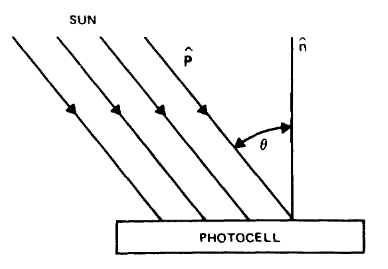
\includegraphics[scale=0.5]{figs/Detector Cossenoildal Sensor Solar.png}
\caption{Sensor Solar de Detecção Cossenoidal}
{Fonte: \cite[p.~156]{wertz2012spacecraft}}
\label{fig:4}
\end{figure}

Para esse modelo, as perdas devido a reflexão de Fresnel, a área efetiva da célula e a reflexão da interface célula-ar dependente do angulo são omitidas.

Para um cubeSat com as células fotovoltaicas encontradas nas seis faces do veículo espacial,  $cos\theta$ pode ser encontrado pela relação do vetor normal do painel $\vec{n}$, com o vetor que aponta para o sol pelo regencial do corpo $\vec{s}^b_{ib}$, sendo ambos unitários.

\begin{equation}
I(\theta)=I(0)cos\theta
\end{equation}
\begin{equation}
I(\theta)=I(0)\vec{n}^T \vec{s}_b
\end{equation}
Utilizando a mesma metodologia para as seis faces tem-se:

\begin{equation}
\mathbf{I}=I(0)\mathbf{N}^T\vec{s}_b
\end{equation}

Sendo $\mathbf{N}$:

\begin{equation}
\mathbf{N}=\begin{bmatrix}
1 & 0 & 0 & -1 & 0 & 0\\ 
0 & 1 & 0 & 0 & -1 & 0\\ 
0 & 0 & 1 & 0 & 0 & -1
\end{bmatrix}\end{equation}

Mas ainda $\vec{s}^b_{ib}$ pode ser encontrado por:

\begin{equation}
\vec{s}_b=C^{B/I}\vec{s}_i\\
\end{equation}
Por fim tem-se:
\begin{equation}
\mathbf{I}=I(0)\mathbf{N}^T C^{B/I}\vec{s}_i
\end{equation}

O sensor magnético ou magnetômetro, fornece a medida do campo magnético terrestre em três eixos. É necessário atenção para o tratamento de ruídos, já que correntes elétricas, campos magnéticos e temperatura, produzidas externas ou internas ao CubeSat interferem nas medições.

Análogo ao caso anterior as medidas do sensor magnético serão dadas utilizando o sistema de referência o de coordenadas do corpo. 

Utilizando um modelo de dipolo inclinado para o campo magnético da terra, é possível escrever seus componentes no SCGI como:

\begin{equation}
m_i^* = \frac{R_T^3H_0}{r^3}\left [ 3\mathbf{d}_i^T\mathbf{\hat{r}}_i\mathbf{\hat{r}}_i-\mathbf{d}_i \right ]
\end{equation}

Onde $\mathbf{d}_i$ é a direção unitária do dipolo no referencial inercial:

\begin{equation}
\mathbf{d}_i=\begin{bmatrix} \sin\theta_m'\cos\alpha_m \\\sin\theta_m'\sin\alpha_m \\ \cos\theta_m'\end{bmatrix}
\end{equation}

Substituindo acima:
\begin{equation}
m_i^*=\frac{R_T^3H_0}{r^3}\begin{bmatrix} 3(\mathbf{d}_i^T\mathbf{\hat{r}}_i)\hat{r}_1 -\sin\theta_m'\cos\alpha_m \\ 3(\mathbf{d}_i^T\mathbf{\hat{r}}_i)\hat{r}_2-\sin\theta_m'\sin\alpha_m \\3(\mathbf{d}_i^T\mathbf{\hat{r}}_i)\hat{r}_3-\cos\theta_m'\end{bmatrix}
\end{equation}

\begin{figure}[htpb]
\centering
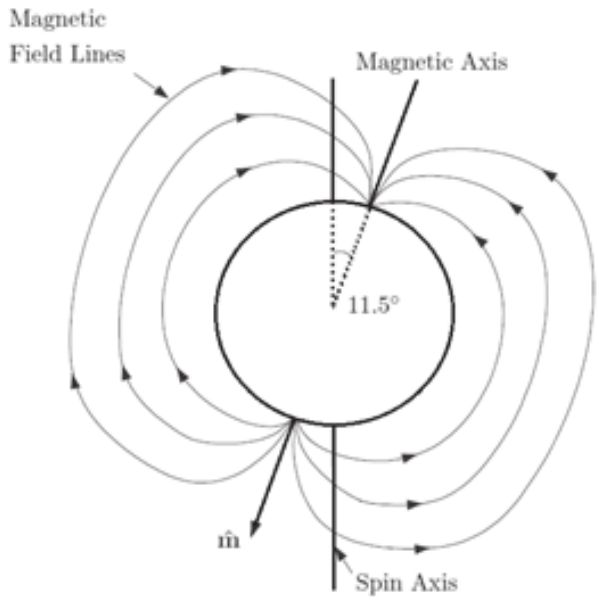
\includegraphics[scale=0.3]{figs/magfield.png}
\caption{Modelo Sensor Magnético}
{Fonte: \cite[p.~13]{mahdi2018attitude}}
\label{fig:5}
\end{figure}

Sendo $r$ o vetor posição do veículo espacial, $R_T$ o raio da Terra, $H_0$ a constante característica do vetor magnético da Terra e $\theta_m'$ co-elevação.

\begin{equation}
\alpha_m = \theta_{go}+\omega_Tt+\phi_m'
\end{equation}

Sendo $\theta_{}go$ a época sideral de greenwich, $\omega_T$ a rotação média da Terra, $t$ o tempo desde a época e $\phi_m'$ a longitude leste do dipolo.

O girômetro do inglês (\textit{rate gyro}) são dispositivos que medem a velocidade angular de um objeto em rotação, esses sensores tem opções mais simples e baratas geralmente adequadas para o controle da taxa de rotação de um cubeSat mas em um sistema com feedback sua saída requer correção frequente para determinação usando outros sensores como solares e magnéticos.
 
(COMPLEMENTAR)

\subsection{Determinação de Atitude: Método TRIAD}\label{sec:3.1.5}

Pelo menos dois vetores são necessários para determinar a atitude. No entanto, é importante notar que, embora sejam necessários três parâmetros independentes para determinar a atitude, cada medição de vetor unitário na verdade fornece apenas dois parâmetros devido à restrição do vetor unitário. Portanto, são necessários três escalares para determinar completamente a atitude. Assim, a exigência é de mais de uma, mas menos de dois medições de vetores. A determinação da atitude é única nesse sentido, pois uma medição não é suficiente, ou seja, o problema é subdeterminado, e duas medições são demais, ou seja, o problema é super-determinado. A principal implicação dessa observação é que todos os algoritmos de determinação de atitude são realmente algoritmos de estimação de atitude.

O algoritmo TRIAD é uma técnica fundamental na determinação da atitude de uma espaçonave. A atitude de uma espaçonave é essencialmente a descrição da matriz de rotação que descreve a orientação do referencial fixo à espaçonave, $B$, em relação a um referencial conhecido, como um referencial inercial, $I$.

Embora essa matriz de cossenos diretores possua nove números, como mostrado anteriormente, apenas três números são necessários para determiná-la completamente. Como cada vetor unitário medido fornece duas informações, são necessárias pelo menos duas medidas diferentes para determinar a atitude o que resulta em um problema super-determinado, pois temos três incógnitas e quatro quantidades conhecidas.

O algoritmo TRIAD parte de dois vetores de medição, como a direção para o sol e a direção do campo magnético terrestre. Denotamos os vetores reais como $\vec{s}$ e $\vec{m}$, respectivamente. As componentes medidas dos vetores, em relação ao referencial do corpo, são denotadas por $\vec{s}_b$ e $\vec{m}_b$, respectivamente. As componentes conhecidas dos vetores no referencial inercial são $\vec{s}_i$ e $\vec{m}_i$.

Idealmente, a matriz de rotação, ou matriz de atitude, $C^{B/I}$, satisfaz $\vec{s}_b=C^{B/I}\vec{s}_i$ e $\vec{m}_b=C^{B/I}\vec{m}_i$. Infelizmente, como o problema é super-determinado, geralmente não é possível encontrar tal $C^{B/I}$. O algoritmo de determinação de atitude determinística mais simples é baseado em descartar uma parte dessa informação no entanto, essa abordagem não se resume simplesmente a descartar uma das componentes de uma das direções medidas. O algoritmo é conhecido como algoritmo TRIAD, porque é baseado na construção de dois triângulos de vetores unitários ortogonais usando as informações vetoriais disponíveis. Os dois triângulos são as componentes do mesmo referencial, denotado por $T$, expresso nos referenciais do corpo e inercial. Este referencial é construído assumindo que um dos pares de vetores corpo/inercial está correto.


\begin{equation}
\begin{bmatrix} \hat{t}_1 \\ \hat{t}_2 \\ \hat{t}_3
\end{bmatrix} = \begin{bmatrix} \hat{s} \\  \hat{s}\times\hat{m} 
\\ \hat{t}_1\times\hat{t}_2
\end{bmatrix}
\end{equation}

\begin{equation}
\begin{bmatrix} \hat{t}_{1b} \\ \hat{t}_{2b} \\ \hat{t}_{3b}
\end{bmatrix} = \begin{bmatrix} \hat{s}_b \\  \hat{s}_b\times\hat{m}_b 
\\ \hat{t}_{1b}\times\hat{t}_{2b}
\end{bmatrix}
\end{equation}

\begin{equation}
\begin{bmatrix} \hat{t}_{1i} \\ \hat{t}_{2i} \\ \hat{t}_{3i}
\end{bmatrix} = \begin{bmatrix} \hat{s}_i \\  \hat{s}_i\times\hat{m}_i
\\ \hat{t}_{1i}\times\hat{t}_{2i}
\end{bmatrix}
\end{equation}

\begin{equation}
C^{B/I} = C^{B/T}C^{B/I}=\left [\hat{t}_{1b} \hat{t}_{2b} \hat{t}_{3b}  \right ]
\begin{bmatrix} \hat{t}_{1i}\\\hat{t}_{2i}\\\hat{t}_{3i}
\end{bmatrix}
\end{equation}

\subsection{Controle de Atitude: Técnica de Controle PID}\label{sec:3.1.6}

Para o controle da atitude do CubeSat por rodas de reação se usa um controlador automático estes comparam o valor de saída, medido por um sensor, com o valor de entrada, de referência, desejado. A comparação desses dois valores determina um desvio chamado de erro, e esse sinal de erro é tratado pelo controlador que gera por fim um sinal de controle para os atuadores que agiram sobre o sistema na busca de diminuir esse desvio. A técnica aqui demostrada está presente em \cite[p.~21]{ogata2011engenharia}.

O controle proporcional-integral-derivativo ou PID, é um controle automático que combina ações de natureza proporcional, integral e derivativa no tratamento do sinal de erro. Essa ação combinada oferece as vantagens induviais de cada um desses tipo de controle. 
A utilização de rodas de reação quando o controle é feito por velocidade, no presente caso aplica-se um controlador PID ao sinal de corrente. Dessa forma a equação do sinal de controle é dada por:

\begin{equation}
u(t)=K_p\left(e(t)+\frac{1}{T_i}\int_{0}^{t}e(t)dt+T_d\frac{\mathrm{d}e(t) }{\mathrm{d} t}\right )
\end{equation}

Onde $e(t)$ é o erro entre a velocidade angular de referência e a observada, $K_p$ é o ganho proporcional, $T_i$ é o tempo integrativo e $T_d$ é o tempo derivativo.

Para o caso que o modelo matemático da planta a ser considerada possa ser obtido, então é possível aplicar técnicas de projeto para auxiliar na determinação de parâmetros do controlador para atender as especificações do regime transitório e do regime permanente do sistema de malha fechada. Contudo se a planta for muito complexa é possível que a abordagem analítica seja não praticável, assim tem-se que recorrer para uma abordagem experimental de sintonia do controlador PID.

O método de sintonia  de Ziegler e Nichols, \cite[p.~524]{ogata2011engenharia}, sugere ajustar os parâmetros $Kp$, $T_i$ e $T_d$ a partir da resposta experimental ao aumentar o valor de $K_p$ até resultar em uma estabilidade marginal, quando só a ação proporcional é considerada. Ou seja, definindo $T_i=\infty$ e $T_d=0$, aumenta-se o valor de $K_p$ de 0 até o valor crítico $K_{cr}$no qual a saída oscila de forma sustentada pela primeira vez, o período de oscilação encontrado é $P_{cr}$. Caso para qualquer valor de $K_p$ não se encontre uma resposta oscilatória sustentada do sistema então o método não se aplica.

Para os valores de $P_{cr}$ e $K_{cr}$encontrados Ziegle e Nichols sugere escolher os parâmetros $Kp$, $T_i$ e $T_d$ de acordo com a  tabela~\ref{tab:1} a seguir:

\begin{table}[htpb]
\centering
\caption{Regra de sintonia de Ziegler-Nichols baseada no ganho crítico $K_{cr}$ e no período crítico $P_{cr}$.}\label{tab:1}
\begin{tabular}{|c|c|c|c|}
\hline
\small{Tipo de controlador} & \small{$K_p$} & \small{$T_i$} & \small{$T_d$} \\ \hline
P&$0,5K_{cr}$&$\infty$&$0$\\\hline
PI& $0,45K_{cr}$&$\frac{1}{1,2}P_{cr}$&$0$\\\hline
PID	& $0,6K_{cr}$&$0,5P_{cr}$&$0,125P_{cr}$\\\hline
\end{tabular}
\end{table}


\subsection{Rodas de Reação em 3 Eixos}\label{sec:3.1.6.1}


As rodas de reação (RDR) são dispositivos atuadores utilizados para o controle de atitude de veículos espaciais, possuindo, como a base de seu funcionamento, a transferência de momento angular. Podendo ser arranjadas em conjuntos de três unidades para controlar a rotação nos três eixos, de quatro unidades para além dos controles dos três eixos oferecer redundância ao sistema, ou avulso.

Por permitirem a correção de atitude com precisão, estes dispositivos têm operação mais complexa e são mais custosos. Apenas em missões nas quais os requisitos do apontamento são mais sensíveis se utiliza esse tipo de atuador, sendo assim menos comuns em CubeSats.

Contudo, com o aumento de missões mais rebuscadas, estas que se encontram distante do campo magnético da Terra, faz-se mais necessário esses dispositivos, deste modo, se tornando comuns e até comercializados, que é o caso da SatBus 4RW0, um conjunto de 4 rodas de reação desenvolvidas pela NanoAvionics para seus CubeSats (M3P ao M16P),  também podendo ser encomendadas, e a CubeWhell encontrada na CubeSat Shop e a Blue Canyon com sistemas completamente integrados de ADCS com rodas de reação acopladas,  Figura~\ref{fig:10}.


Uma roda de reação é uma massa rotativa motorizada que fornece torque para manobra e é usada para o apontamento de satélites. Podendo rotacionar tanto no sentido horário quanto no anti-horário, assim como acelerar ou desacelerar, criando torques e manobrando o satélite.

Esse dispositivo necessita de uma forma de dessaturar ao longo do tempo, assim um sistema adicional podendo ser torqueadores magnéticos ou propulsores cumprem essa função descarregando o momento angular.

Mais precisamente uma roda de reação consistem em cilindros de metal encaixadas em um motor sem escova achatado, é indispensável que esse motor tenha uma boa relação potência consumo e que funcione dentro da faixa de potência oferecida por esse sistema do satélite. Estas rodas de reação permitem um alto grau de acurácia e são essenciais em missões as quais um controle mais fino e robusto é necessário.

Variando entre 0,4 a 40 $\frac{kg\;m^2}{s}$, podendo ser uma roda pequena e rápida ou uma roda grande e lenta. Esses dispositivos se baseiam no principio da conservação de momento, \textit{i.e.}, $\vec{H}=J^b_{RDR}\;\vec{\omega}_{RDR}$. Onde $\vec{\omega}_{RDR}$ é o vetor das velocidades angulares e $J^b_{RDR}$ a matriz de inércia da roda-de-reação. O modelo utilizado para a caracterização física-matemática da roda de reação foi adaptado de \cite[p.~270-271]{wertz2012spacecraft}.

O torque da roda é oferecido por um motor de indução elétrica de corrente contínua, alimentado por pulsos quadrados provenientes da bateria controlados pelo computador de bordo ao nível do ciclo de trabalho, que está relacionado com a velocidade de rotação da roda.

O Ciclo de trabalho $X_{ct}$ varia entre +1 e -1 a partir do sinal de controle, $V$, mostrado na Figura~\ref{fig:14}.

\begin{figure}[htpb]
\centering
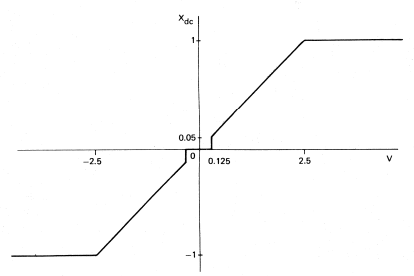
\includegraphics[scale=1]{figs/CicloTrabalho.png}
\caption{Ciclo de Trabalho $X_{CT}$}
{Fonte: \cite[p.~271]{wertz2012spacecraft}}
\label{fig:6}
\end{figure}

O torque líquido é encontrado por:

\begin{equation}N=X_{ct}N_{em}-N_{fricção}\end{equation}

Onde $N_{em}$ é o torque eletromagnético produzido por indução, e $N_{fricção}$ contabiliza o atrito viscoso e de Coumlomb, descrito por:

\begin{equation}N_{fricção}=N_c\left (\frac{s}{|s|}\right )+f\;s\end{equation}

Onde $N_c$ é o coeficiente de fricção de Coulomb, $f$ é o coeficiente de fricção viscosa e $s$ a velocidade de rotação da roda.

Para encontrar o torque eletromagnético, $N_{em}$, pode-se se utilizar a seguinte aproximação:

\begin{equation} N_{em} = \frac{2N_0\alpha\;r}{(\alpha^2+r^2)}\end{equation}

Sendo, $N_0$ a magnitude máxima de $N_{em}$, $\alpha$ é o valor de $r$ onde se encontra $N_0$ e $r$ é encontrado pela seguinte relação:

\begin{equation}r=1-\frac{s}{s_{max}}\;\text{para}\;X_{ct}>0 \end{equation}\begin{equation} r=1+\frac{s}{s_{max}}\;\text{para}\;X_{ct}<0\end{equation}

Atente-se que $s_{max}$ é conhecida pela velocidade de sincronização da roda-de-reação. O torque eletromagnético em relação a velocidade da roda é mostrado na Figura~\ref{fig:15}.

\begin{figure}[htpb]
\centering
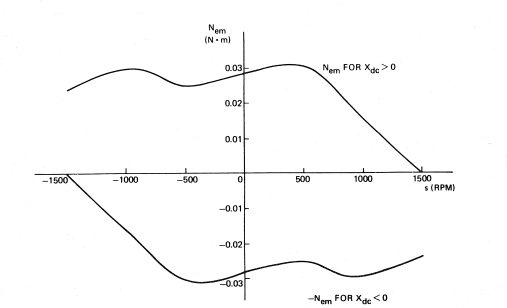
\includegraphics[scale=1]{figs/torqueEletromagnetico.png}
\caption{Torque Eletromagnético $N_{em}$ em relação a velocidade de rotação da roda-de-reação $s$}
{Fonte: \cite[p.~271]{wertz2012spacecraft}}
\label{fig:15}
\end{figure}

\subsection{Modelagem das Rodas-De-Reação}\label{sec:3.1.6.2}

A equação para uma roda-de-reação, controlada por uma corrente contínua $i(t)$ ao invés de uma tensão de controle, e, utilizando os modelos de zona ociosa,  torque eletromagnético, fricção viscosa e o coeficiente do torque de Coulomb descritos acima, é dada por:

\begin{equation}
T_{aplicado}=J_{axial}\frac{d\omega_{rdr}}{dt}=Xct(i(t))\frac{2N_0\alpha\left (1-\frac{\omega_{rdr}}{\omega_{rdr\;max}} \right )}{\alpha^2\left (1-\frac{\omega_{rdr}}{\omega_{rdr\;max}} \right )^2}-\left (sign(Xct(i(t)))N_c+f\omega_{rdr}\right )
\end{equation}
Como as três rodas-de-reação são idênticas, pode-se modela-las como cilindros de metal com massa uniformemente distribuída, onde $m_{rdr}$ é a massa e $\{\rho_{rdr}\}$ o raio:

\begin{equation}{J_{axial}}=\frac{m}{2}\rho^2_{rdr}\end{equation}Contabilizando somente as componentes axiais das rodas de reação e alinhando cada com eixos principais de inercia da matriz de inércia coincidentes ao sistema de referencia fixa no corpo, tem-se que   $J^b_{rdr}$:

\begin{equation}J^b_{rdr} =\begin{bmatrix}
{J_{axial}}_1&0&0 \\0 &{J_{axial}}_2&0 \\ 0&0&{J_{axial}}_3
\end{bmatrix}\end{equation}E aplicando a modelagem para cada eixo, tem-se que o vetor de torques aplicado fica:
\begin{equation}
\vec{T}_{aplicado}=J^b_{rdr}\frac{d\vec{\omega^b_{rdr}}}{dt}
\end{equation}




% PARTE
\part{Proposta}
\chapter{Implementando Laboratório Virtual}\label{cap:proposta}

O presente projeto propõe o desenvolvimento de um laboratório virtual como de ambiente para o ensino de modelagem e controle de CubeSats por meio de simulação. Utilizando ferramentas aberta e livres contornando o problema de custo. E de roteiros para instalação, configuração e uso, contornando o problema da curva de aprendizado.

\section{Requisitos}\label{Requisitos}

Para a realização do presente projeto está foi escolhido as aplicações a seguir:

\begin{itemize}
    \item Ubuntu 24.04 LTS
    \item JSBSim
    \item FlightGear
    \item Python
    \item Blender
\end{itemize}

O JSBSim é uma plataforma de código aberto para modelagem de dinâmica de voo, simulando a física e a matemática dos 6 graus de liberdade do movimento de aeronaves, foguetes e outros veículos aéreos. Ela pode ser executada independentemente ou integrada a outros simuladores como o FlightGear, \citeonline{manualJSBSim}.

O FlightGear por sua vez é um simulador de voo gratuito e de código aberto que oferece uma experiência realista de voo para várias plataformas incluindo o Windows, macOS e Linux podendo ser usado para pesquisa. Quando integrado ao JSBSim ele oferece uma interface visual, permitindo visualizar o comportamento de uma aeronave simuladas, \citeonline{manualFlightGear}.

Ambos programas são escritos em C++, mas possuem integração com o Python, os modelos das aeronaves são descritos em XML, onde é incluído propriedades inerciais, modelos aerodinâmicos, sistema e componentes.

Para o funcionamento é previsto o hardware mínimo a seguir:

\begin{itemize}
    \item Memória: 4 GB
    \item Disco: SSD 120 GB
    \item Placa de Vídeo: 1GB Dedicada
    \item Processador: QuadCore 2.1 GHz
\end{itemize}

É possível encontrar em suas respectivas páginas oficiais de forma, o sistema operacional Ubuntu, o modelo de dinâmica de voo JSBSim e o simulador de voo FlightGear.

\section{CubeSat Design}

Define-se o cubesat como um corpo rígido homogêneo, o mesmo 10 cm de comprimento, 20 cm de lagura e 30 cm de altura e 5kg de massa.

Considerando que o eixo do corpo está alinhado com os eixos principais de Inércia, tem-se:

\begin{verbatim}
<mass_balance>
	<ixx unit="KG*M2"> 0.05416667 </ixx>
	<iyy unit="KG*M2"> 0.04166667 </iyy>
	<izz unit="KG*M2"> 0.02083333 </izz>
	<ixy unit="KG*M2"> 0 </ixy>
	<ixz unit="KG*M2"> 0 </ixz>
	<iyz unit="KG*M2"> 0 </iyz>
	<emptywt unit="KG"> 5 </emptywt>
	<location name="CG" unit="M">
		<x> 0 </x>
		<y> 0 </y>
		<z> 0 </z>
	</location>
</mass_balance>

\end{verbatim}

Define-se a roda de reação como um corpo rígido homogêneo cilíndrico, de raio 0.0435 m e massa de 0.137kg.

Considerando que o eixo do corpo está alinhado com os eixos principais de Inércia, tem-se:

\begin{verbatim}
<!-- ROTATION IN X -->
	<force name="RDR_x_1" frame="BODY">
	<function>
		<property> actuator/RDR-x </property>
	</function>
	<location unit="M">
		<x>0</x>
		<y>0</y>
		<z>0.5</z>
	</location>
	<direction>
		<x>  0 </x>
		<y>  1 </y>
		<z>  0 </z>
	</direction>
</force>

<force name="RDR_x_2" frame="BODY">
	<function>
		<property> actuator/RDR-x </property>
	</function>
	<location unit="M">
		<x>0</x>
		<y>0</y>
		<z>-0.5</z>
	</location>
	<direction>
		<x>  0 </x>
		<y> -1 </y>
		<z>  0 </z>
	</direction>
</force>
\end{verbatim}

Perceba que para caracterização devida do momento é feita um binário de força.

\section{Considerações Finais}





% PARTE
\part{Parte Final}
\chapter{Cronograma de Atividades}\label{cap:resultados}

\section{Atividades Previstas}
\begin{enumerate}

    \item Exame de Qualificação de Mestrado do PPGMEC (Data 23/04/2024)
    \item Roteiro 3: Adicionando Atuadores - ROS2 Control 
    \item Roteiro 4: Determinação e Controle de Atitude
    \item CONEM 2024 (29/07/24 a 02/08/24)
    \item Defesa da Dissertação de Mestrado (Previsão 2024.03)
    
\end{enumerate}

\section{Cronograma}


\noindent\begin{ganttchart}[y unit title=0.5cm,
y unit chart=0.5cm,
vgrid,hgrid,
title height=1,
bar/.style={draw,fill=cyan},
bar incomplete/.append style={fill=yellow!50},
bar height=0.5]{1}{12}
 \gantttitle{2024.1}{4} \gantttitle{2024.2}{4}  \gantttitle{2024.3}{4} \\
 \gantttitlelist{1,...,4}{1} \gantttitlelist{5,...,8}{1}  \gantttitlelist{9,...,12}{1}\\
 \ganttbar{Qualificação}{4}{4} \\
 \ganttbar{Roteiro 3}{5}{7} \\
 \ganttbar{Roteiro 4}{5}{7} \\
 \ganttbar{CONEM 2024}{8}{8} \\
 \ganttbar{Defesa}{12}{12}
 % rela\c c\~oes
% \ganttlink{elem2}{elem3}
\end{ganttchart}
\chapter*{Conclusões e Trabalhos Futuros}\label{cap:conclusao}
\addcontentsline{toc}{chapter}{Conclusão e Trabalhos Futuros}

\lipsum[81]

\section*{Conclusões}

\lipsum[82-84]

\section*{Trabalhos Futuros}

\lipsum[85] 

% ----------------------------------------------------------
% ELEMENTOS PÓS-TEXTUAIS (Referências, Glossário, Apêndices)
% ----------------------------------------------------------
\postextual

% Referências bibliográficas
\bibliography{bibliografia}

% Glossário (Consulte o manual)
%\glossary

% Apêndices
% ----------------------------------------------------------
% Apêndices
% ----------------------------------------------------------

% ---
% Inicia os apêndices
% ---
\begin{apendicesenv}

% Imprime uma página indicando o início dos apêndices
\partapendices

% ----------------------------------------------------------
\chapter{Primeiro Apêncice}
% ----------------------------------------------------------

\lipsum[50] % Texto qualquer. REMOVER!!

% ----------------------------------------------------------
\chapter{Segundo apêndice com título tão grande quanto se queira porque ele já faz a quebra de linha da coisa toda}
% ----------------------------------------------------------
\lipsum[51-53] % Texto qualquer. REMOVER!!

\end{apendicesenv}
% ---

% Anexos
% ----------------------------------------------------------
% Apêndices
% ----------------------------------------------------------

% ---
% Inicia os anexos
% ---
\begin{anexosenv}

% Imprime uma página indicando o início dos anexos
\partanexos

% ---
\chapter{Nome do Primeiro Anexo}
% ---
\lipsum[30] % Texto qualquer. REMOVER!!

% ---
\chapter{Nome de Outro Anexo}
% ---

\lipsum[32] % Texto qualquer. REMOVER!!

\end{anexosenv}

% Índice remissivo (Consultar manual)
%\phantompart
%\printindex

\end{document}
